\documentclass[11pt]{report}
\usepackage[margin=1in]{geometry}
\usepackage{titlesec}
\usepackage{graphicx}
\usepackage{parskip}
\usepackage{glossaries}
\usepackage{datetime}

\titleformat{\chapter}{\Large\bfseries}{}{0pt}{\huge}
\titlespacing\chapter{0pt}{*1}{*1}
\titlespacing\section{0pt}{*0}{-\parskip}
\titlespacing\subsection{0pt}{*0}{-\parskip}
\titlespacing\paragraph{0pt}{*0}{*3}

\newcommand*{\TitleFont}{
      \usefont{\encodingdefault}{\rmdefault}{b}{n}
      \fontsize{24}{36}
      \selectfont
}
\newcommand{\thickline}{\rule{\textwidth}{1.6pt}}
\newcommand{\thinline}{\rule{\textwidth}{0.4pt}}
\newcommand{\novspace}{\vspace*{-\baselineskip}\vspace*{4pt}}
\renewcommand{\dateseparator}{-}
\let\oldtitle\title
\renewcommand{\title}[1]{\oldtitle{\thickline \\ \novspace \thinline \\ \TitleFont {#1} \thinline \\ \novspace \thickline}}
\newcommand{\tableoffiguresandtables}{\listoffigures\begingroup\let\clearpage\relax\listoftables\endgroup}

\author{
	Evan Milton \\
	Computer and Electronics Engineering \\
	University of Nebraska at Lincoln - Omaha Campus \\
	Electronics Engineering
		\and
	Josh DeWitt \\
	Computer and Electronics Engineering \\
	University of Nebraska at Lincoln - Omaha Campus \\
	Computer Engineering and Mathematics, minor in Computer Science
		\and
	Chad Staley \\
	Computer and Electronics Engineering \\
	University of Nebraska at Lincoln - Omaha Campus \\
	Electronics Engineering
		\and
	James Gehringer \\
	Computer and Electronics Engineering \\
	University of Nebraska at Lincoln - Omaha Campus \\
	Computer Engineering, minor in Computer Science
}
\date{\yyyymmdddate\today}

\newacronym{2d}{2-D}{Two-Dimensional}
\newacronym{3d}{3-D}{Three-Dimensional}
\newacronym{aon}{AON}{Activity On Node}
\newacronym{arm}{ARM}{Advanced RISC Machines}
\newacronym{bom}{BOM}{Bill of Materials}
\newacronym{cad}{CAD}{Computer-Aided Design}
\newacronym{ceen}{CEEN}{Computer and Electronics Engineering}
\newacronym{ceenc}{\textsc{CeeNC}}{\gls{ceen} Numerical Controller}
\newacronym{cnc}{CNC}{Computer Numerical Control}
\newacronym{cpu}{CPU}{Central Processing Unit}
\newacronym{dmm}{DMM}{Digital Multi-Meter}
\newacronym{drc}{DRC}{Design Rules Check}
\newacronym{dvi}{DVI}{Digital Visual Interface}
\newacronym{eco}{ECO}{Engineering Change Order}
\newacronym{ecr}{ECR}{Engineering Change Request}
\newacronym{emi}{EMI}{Electromagnetic Interference}
\newacronym{fifo}{FIFO}{First-In, First-Out}
\newacronym{fmeca}{FMECA}{Failure Mode, Effects, and Criticality Analysis}
\newacronym{gpio}{GPIO}{General Purpose Input/Output}
\newacronym{ieee}{IEEE}{Institute of Electrical and Electronics Engineers}
\newacronym{i2c}{I$^2$C}{Inter-Integrated Circuit}
\newacronym{jtag}{JTAG}{Joint Test Action Group}
\newacronym{kb}{kB}{kiloBytes}
\newacronym{led}{LED}{Light Emitting Diode}
\newacronym{lrc}{LRC}{Linear Responsibility Chart}
\newacronym{mpe}{MPE}{Maximum Permissible Exposure}
\newacronym{mttf}{MTTF}{Mean Time to Failure}
\newacronym{nesc}{NESC}{National Electrical Safety Code}
\newacronym{os}{OS}{Operating System}
\newacronym{otp}{OTP}{One-Time Programmable}
\newacronym{pcb}{PCB}{Printed Circuit Board}
\newacronym{pi}{Pi}{Raspberry Pi}
\newacronym{pcsc}{PCSC}{Project Common Success Criteria}
\newacronym{pssc}{PSSC}{Project Specific Success Criteria}
\newacronym{ram}{RAM}{Random Access Memory}
\newacronym{rom}{ROM}{Read-Only Memory}
\newacronym{rf}{RF}{Radio Frequency}
\newacronym{spi}{SPI}{Serial Peripheral Interface}
\newacronym{ssh}{SSH}{Secure Shell}
\newacronym{sar}{SAR}{Specific Absorption Rate}
\newacronym{smt}{SMT}{Surface Mount Technology}
\newacronym{tcpip}{TCP/IP}{Transmission Control Protocol/Internet Protocol}
\newacronym{ti}{TI}{Texas Instruments}
\newacronym{uart}{UART}{Universal Asynchronous Receiver/Transmitter}
\newacronym{wbs}{WBS}{Work Breakdown Structure}
\newacronym{xp}{XP}{Extreme Programming}

\titleandsubtitle{CNC Interface \\ Project Final Report}{Submitted in Partial Fulfillment of the Requirements for the B.Sc. Degree, \\ Computer and Electronics Engineering, College of Engineering, \\ University of Nebraska \\ Peter Kiewit Institute, Omaha, Nebraska, U.S.A}

\begin{document}
\maketitle
\tableofcontents
\tableoffiguresandtables

\chapter{Front Matter}
\textbf{Ethical Design Statement}

As the CeeNC was developed, the IEEE Code of Ethics was reviewed and considered when decisions were made.
The CeeNC is designed to be safe for all users.

\textbf{Environmental Impact Statement}

The environmental impact of the CeeNC was strongly considered during development. 
The CeeNC is designed to keep its environmental impact minimal, eliminating toxic materials by using lead-free fabricators.

\section{Abstract}




\section{Acknowledgments}


\chapter{Executive Summary}
\chapter{Introduction}
This is the final report for the senior thesis design course offered by the \gls{ceen} department of the University of Nebraska-Lincoln.
The team chose to design and create a \gls{cnc} interface that has been nicknamed the \gls{ceenc}.

\section{Problem Statement}
The \gls{ceenc} is a web-enabled \gls{cnc} interface designed with students and hobbyists in mind.
Most modern \gls{cnc} interfaces and drivers are large and expensive, making it difficult for students, hobbyists, and smaller companies to own a \gls{cnc}.
The \gls{ceenc} is an affordable and compact device, enabling users to cut down on project development time and cost.
The device can also be configured for multiple setups, including linear \gls{cnc}s, delta robots, or a \gls{3d} printer.
The web interface also improves upon connectivity, allowing the device to be used from anywhere on the network.

\section{Objectives}
The purpose of the \gls{ceenc} project is to create a \gls{cnc} interface, capable of receiving standardized G-code through	 \gls{tcpip}, processing the G-code, and driving motors and general purpose outputs according to the G-code.
G-code is a standard \gls{cnc} programming language, but is more complicated than accepting individual commands to move the motors.
Figure ~\ref{fig:architecture} shows the objective tree for the \gls{ceenc}, showing the importance of safety and \gls{cnc} functionality.
The numbers referencing \gls{pssc}s are described in ~\ref{sec:psscs}.

\begin{figure}[h]
	\centering
	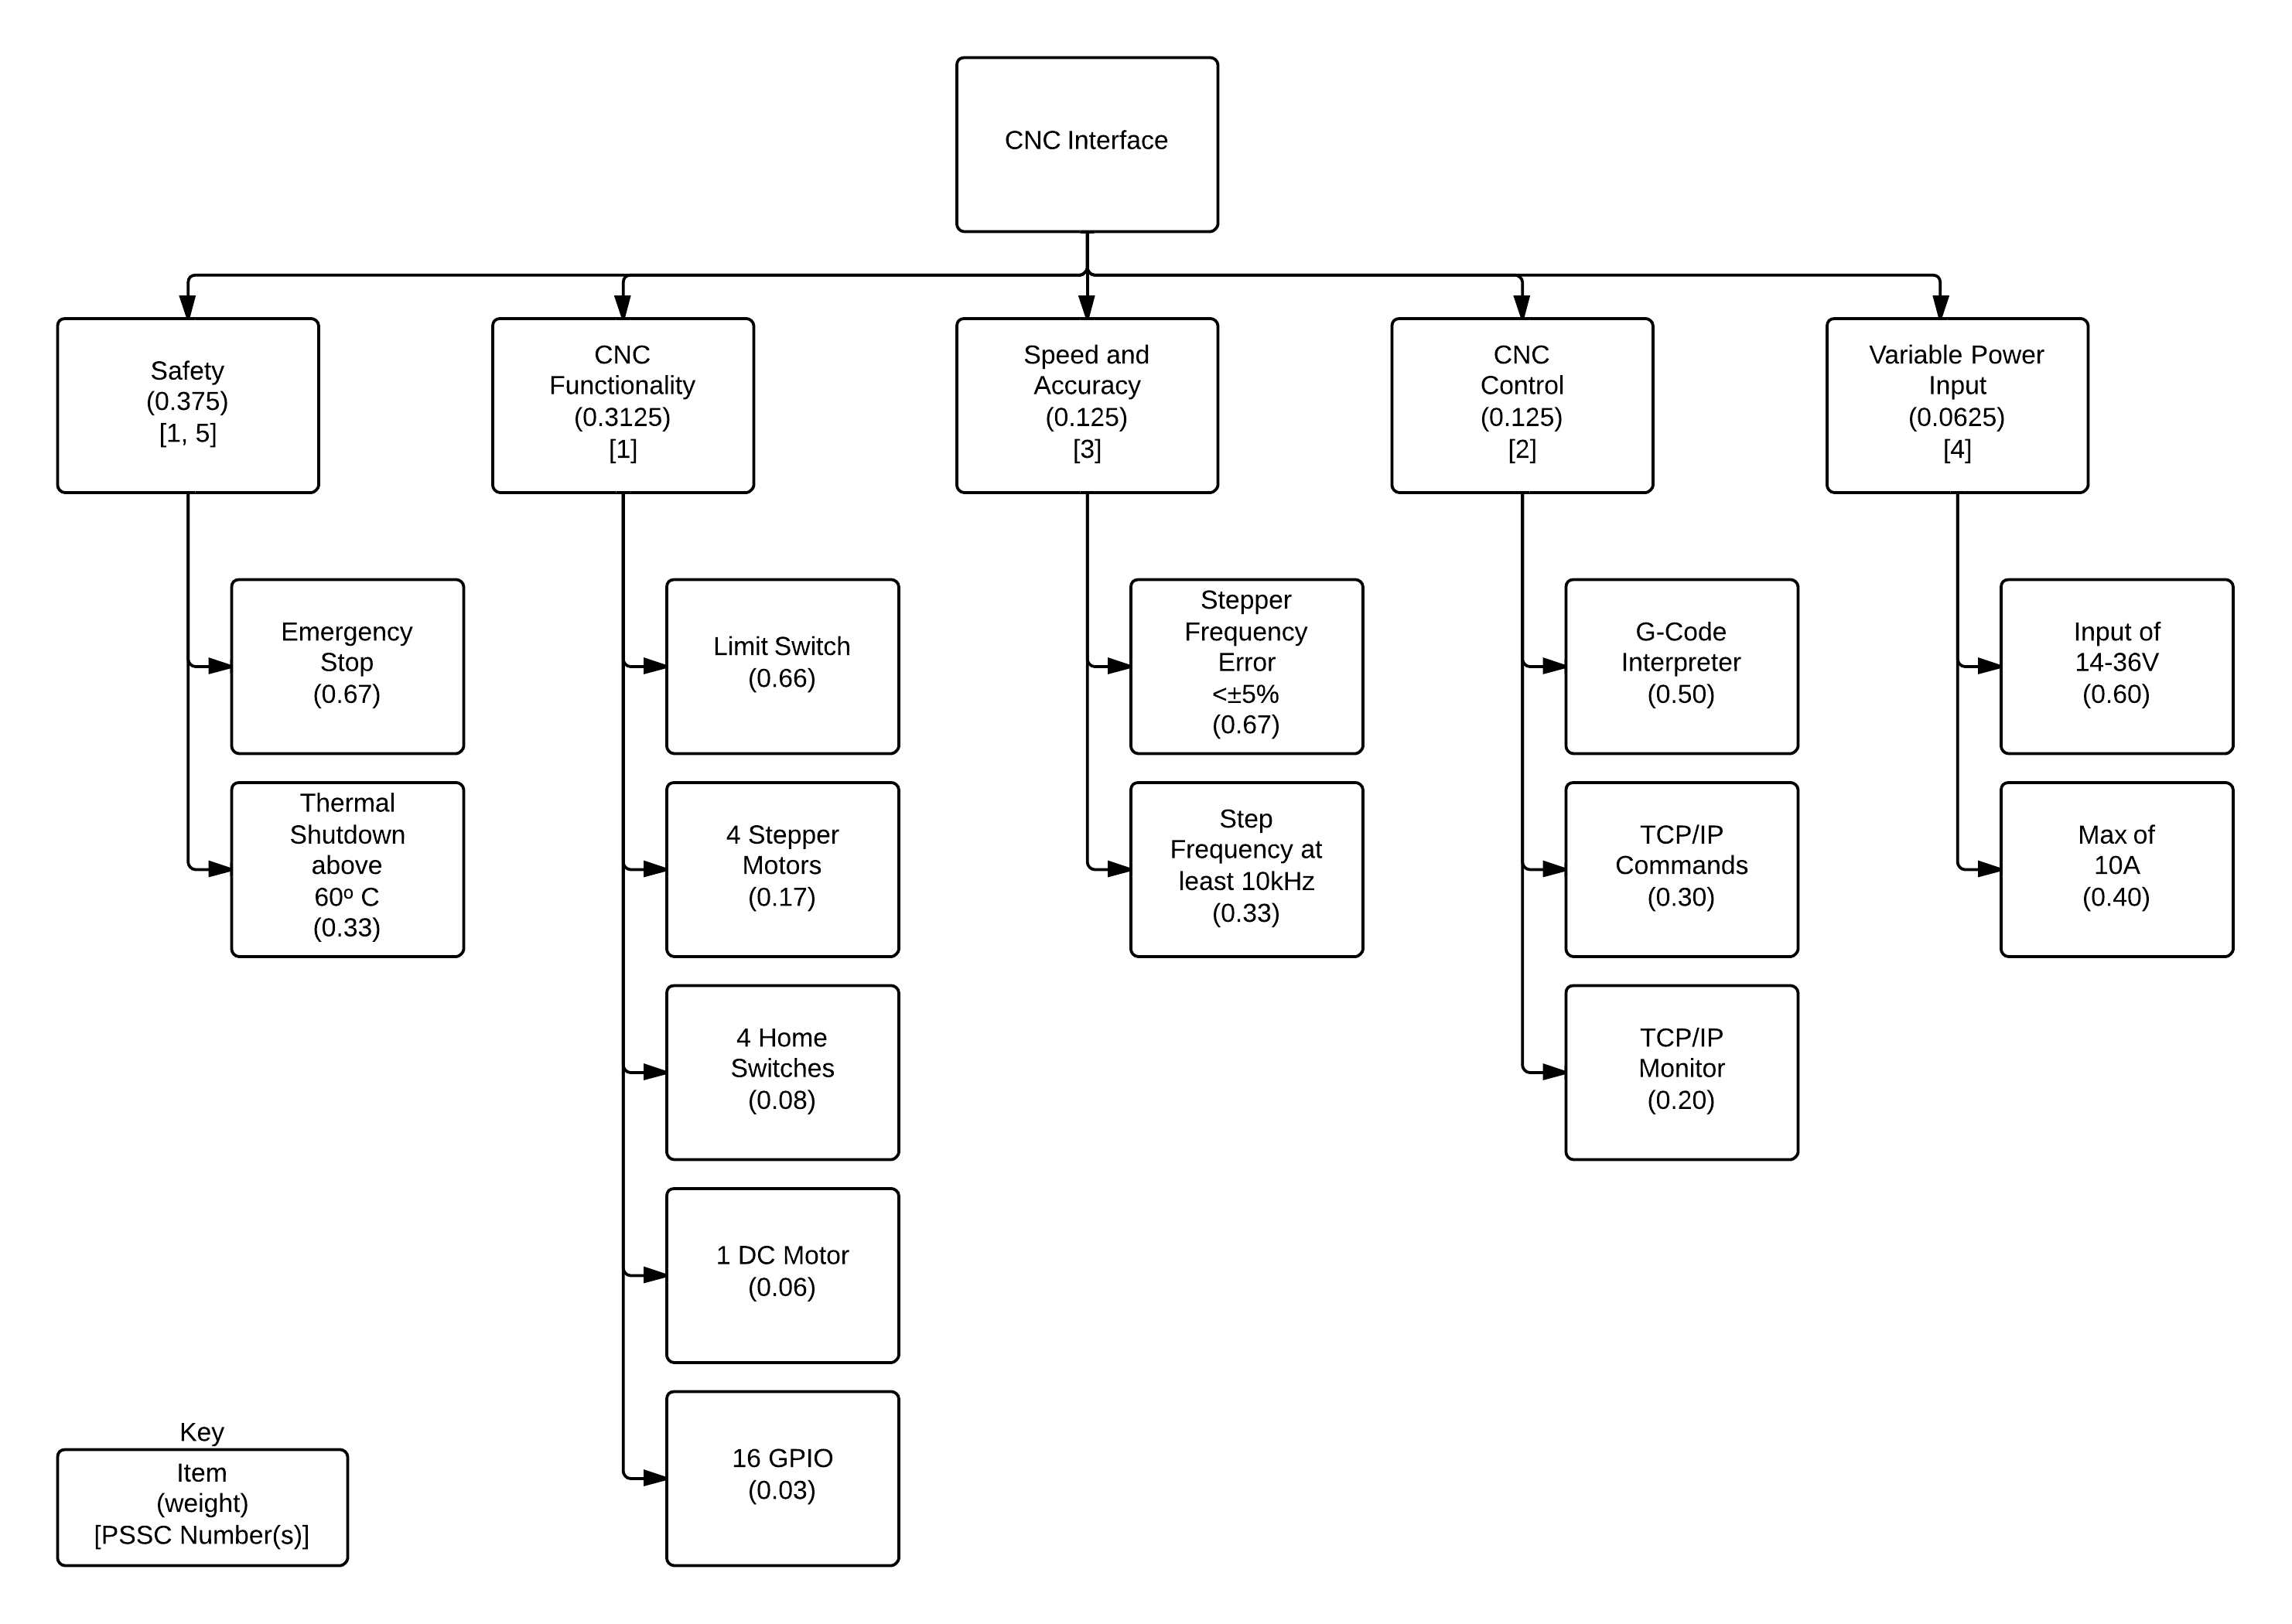
\includegraphics[width=1\textwidth]{objective-tree.png}
	\caption{Objective Tree}
	\label{fig:o-tree}
\end{figure}

\section{Report Format}
This report discusses the need for the product, the solution design process, the implemented solution and how it works, and how the solutions may affect the world.
Final recommendations are given for future enhancements for the project to move forward and continue improving.

\chapter{Problem Formulation}

The modern \gls{cnc} interface is limited to use of a full computer system in combination with a motor driver platform.
This setup can cost upwards of \$500, depending on the quality and system specifications, which is not affordable for many students and hobbyists.
Students and hobbyists will benefit from having their own \gls{cnc}.
The \gls{ceenc} will encapsulate the hardware and software required for a \gls{cnc} in a user-friendly and compact design for less than \$100, bringing the \gls{cnc} interface to a price point comparable with that of the modern printer.

\section{Background}
Most \gls{3d} printers or \gls{cnc} mills come with software interfaces to control the printers.
Once the software is installed on a computer, files can be made and uploaded for printing.
The limitation of this model is that some software is not designed to run on all operating systems and the user must access the \gls{cnc} through the computer that the software is installed on.

\subsection{Competitive Products}
Before beginning design of the \gls{ceenc}, several alternate \gls{cnc} interfaces were analyzed to understand the current standards and user needs.
While several \gls{cnc} interfaces exist, the \gls{ceenc} has added focus on the usability and lower cost than the alternatives.

\subsubsection{MakerBot}
The MakerBot is considered the leader in the current \gls{3d} printer market.
The interface software is MakerBot Desktop, or the older versions were MakerWare.
The MakerBot software allows a user to scan in models and upload files to be printed.
Currently, there is not support for sending files over WiFi, only over USB and Ethernet.
The MakerBot costs around \$2000 depending on the model, although this includes the entire \gls{cnc} machine, not just the driver portion like the \gls{ceenc}.

\subsubsection{SmoothieBoard}
SmoothieBoard is an open source driver system with simplistic interfacing software.
It supports Ethernet connections and the system can be accessed through a browser to upload files to the device.
Once a file is uploaded, a command line interface on the device is used to execute files.
The SmoothieBoard costs \$169.97.

\subsubsection{EMC2}
EMC2, also known as LinuxCNC is a freely available \gls{cnc} interface.
It allows for multiple \gls{cnc} configurations, giving flexibility to people who want to build their own \gls{cnc}s.
EMC2 requires a dedicated Linux-based machine and can only operate through a parallel port connector.

\subsubsection{Rostock}
The Rostock is a delta robot \gls{3d} printer is supported by RepRap, meaning it is a \gls{cnc} that can print many of its own components for making another device. 
The RepRap is estimated to cost \$500 for the hardware for a work area of 8x8x16 inches.
An Arduino handles the G-code processing that is sent to it through USB.
The assembly instructions do refer to their current firmware as “a pretty hacky proof of concept and not a long term solution” [1] though.

\subsubsection{OtherMill}
The OtherMill is a new \gls{cnc} controlled by OtherPlan software that costs \$2199.
It allows users to upload a variety of file types, that is converted into G-code interally.
The device offers a command line interface that allows users to send indiviual commands.
The OtherPlan software only supports Mac OS X and the OtherMill must be connected to this computer through USB.

\subsection{Patent Liability Analysis}
While there is a patent for a generic \gls{cnc} [1], this project does not specify the hardware for a \gls{cnc} so it does not apply to the \gls{ceenc}
G-code was patented by Fanus Ltd [2] on April 1, 1983, but any patent filed before 1994 had a term of 17 years, meaning that the patent expired in 2000.

\subsubsection{Results of Patent and Product Search}
The patents below focus on methods of interaction with a \gls{cnc}.
A search for method based patents was done for patents on control equations, however no patents for control equations on \gls{cnc} devices were found.
These are the areas of highest potential for liability, due to their similarity to popular commercial products.
Several equations and methods used for navigation calculations were found [3], but those applied to transportation, specifically airplanes.

\textbf{Numerical control unit with set amount of execution} \\
\textbf{Publication Number:} US 8036770 B2 \\
\textbf{Filing Date:} April 4th, 2008 \\
\textbf{Condensed Abstract:}
This patent is for a machine that uses numerical controls.
It will start a command or set of commands when its start button is depressed.
It will also suspend execution if there is a change in direction or a non-cutting command is issued.
It will then wait for the start button to be depressed again before resuming operation [4].

\textbf{Approach For Printing To Web Services-Enabled Printing Devices} \\
\textbf{Publication Number:} US 20100225958 A1 \\
\textbf{Filing Date:} March 6th, 2009 \\
\textbf{Condensed Abstract:}
This patent describes a method for retrieving printer data and displaying what functions it has available on a second party application.
A print driver will hold all the information and the information can be requested by the web service.
The web service will then parse this data and show what options the printer has available and allow print jobs to be made.
Then data and options can be sent back to the printer to create and execute print jobs [5].

\textbf{Control device of electric motor} \\
\textbf{Publication Number:} US 8598818 B2 \\
\textbf{Filing Date:} July 29th, 2005 \\
\textbf{Condensed Abstract:}
This patent describes a method of motor control. 
It breaks the control down into three parts, driving, monitoring, and stopping.
It focuses on stopping the motor in a safe matter, by using the monitoring to determine if the motor is operating under safe conditions.
Specifically, it looks at the velocity of a motor to check if it needs to be forcibly stopped when an emergency stop button is pressed [6].

\textbf{SENA Technologies Products} \\
A product search did not turn up any network enabled \gls{cnc} devices, however it did find a series of devices that would allow a company to connect existing devices to their network.
SENA has a series of products that connects an existing \gls{cnc} to the network through Ethernet, WiFi or Bluetooth.
There would be potential for infringement on these devices.
SENA’s United States office declined to comment on any patents being filed on any of their devices.
A patent search ran with SENA being the assignee returned no results on patents related to these products.

\subsubsection{Analysis of Patent Liability}
Looking at the previously mentioned patents and products, there is a high chance of patent infringement.
The first patent discussed is especially worrisome because the claims are similar to our product's intended functionality.
Using standardized G-code to instruct the work head will remain the same because the patent for G-code has expired.
However, this patent holds control of how G-code is used though, with claims mentioning specific command signifiers.
The major differences between \gls{ceenc} and the claims in the first patent are when their product stops and the types of motors used to drive the \gls{cnc}.
While our product does not include the mechanical side of the \gls{cnc}, it is still designed to drive four stepper motors. 
This patent states that it will use servomotors, as shown in their first figure of the patent [Appedix Figure 1]. 
Secondly, their claims state that any time there is a change in the cutting direction or a non-cutting command is sent, the machine will pause and wait for the start button to be pushed again, but the \gls{ceenc} will run a whole batch of control without stopping or prompting for user input.
Overall, this patent is vague system and many of the concepts were created by the team without reference, so the claims were obvious and it is surprising that it was patentable.

Patent two is not as troubling because their claims do state that they will use a print driver. 
Since the \gls{ceenc} will be configurable, our driver will not return to the host the configurations of the printer.
It will make available to the user the options that can be used to configure the printer.
Secondly, their device sent its data to a second party application, but the \gls{ceenc} will send data to the website and be stored on the \gls{ceenc}, with no second party application needed.
Storing and retrieving data are both part of the claims, but are general practices that are used often.
The second patent also covers the claims that state how options will be passed to the system.

The third patent has some potential for issue, but the wording will show some separation. 
While the \gls{ceenc} will monitor the motor, it only stores the position, not the velocity.
Also, a safety switch will stop the motors, but the safety switch will not engage the motor monitoring as mentioned in the patent. 
The \gls{ceenc} will be constantly monitoring the motors during operation.
Lastly, there will be no need to forcibly stop the motors as stated in the third patent because the \gls{ceenc} uses stepper motors to move a work head, which will immediately stop in an emergency.

\subsubsection{Recommendations and Actions Taken}
The first patent is unavoidable because it covers a large area of \gls{cnc}s, even specifying how to use G-code, which is an obvious standard.
Working around this patent will cause the project to be redesigned from scratch.
The difference of the continuous movement versus the start and stop mentioned in the patent is not a large enough difference to be considered different products.
The major difference is that the patent describes use of servo motors and the \gls{ceenc} uses stepper motors, which require substantially different hardware and software.
Because of this difference, there will be no infringement, and if the patent holders claim there is, it will be able to be argued in court. 
At the very least, a settlement can be reached.

The second patent does not show any potential for infringement because the product centers around data being sent through the network using a second party application.
This is substantially different from the \gls{ceenc} architecture.
The patent describes use a standard communication setup to make sure the data is in a correct format for any second party application.
The \gls{ceenc} will work using point-to-point communication, much like the prevalent network-enabled printers today’s world.

The third patent shows little chance for patent infringement also.
While both products drive stepper motors, the way they are driven done is not the same.
The monitoring between both products is also different in method and end results.

\chapter{Design Requirements and Success Criteria}
The project's success will be determined by whether or not the 10 engineering requirements, consisting of 5 \gls{pcsc} and 5 \gls{pssc}, are met.
The \gls{pssc}s were developed based on the objective tree, shown in Figure ~\ref{fig:o-tree}.

\section{Five Project Common Success Criteria}
\begin{enumerate}
	\item Create a complete \gls{bom} and order/sample all parts needed for the design.
	\item Develop complete, accurate, readable schematic of the design, complete with interface loading analysis and interface timing analysis. 
	\item Complete a layout and etch a \gls{pcb}.
	\item Populate and debug the design on a custom \gls{pcb}.
	\item Professionally package the finished product and demonstrate its functionality.
\end{enumerate}

\section{Five Project Specific Success Criteria}
\label{sec:psscs}
\begin{enumerate}
	\item The system will drive at least 4 stepper motors, 1 DC motor, and 16 general purpose outputs.
The system will receive inputs from at least 1 emergency stop switch and 4 stepper motor home inputs.
	\item The system will Receive G-code through \gls{tcpip}.
The system’s software will be developed using IEEE Std 830-1998 Recommended Practice for Software Requirements Specifications.
	\item The step frequency range will be at least 0Hz to 10kHz.
For any chosen frequency in range, the actual step frequency will be within 5\% of the desired frequency.
	\item The system power supply will accept between 14V and 36V and draw a maximum of 10A, including current required for the motors. 
	\item The system will stop all motors and shutdown all microcontrollers if the main microcontroller temperature reaches $60^{\circ}C$ ($140^{\circ}F$).
\end{enumerate}

\section{Design Constraints}
The major design constraints considered in this report are computational requirements, interface requirements, on-chip peripheral requirements, off-chip peripheral requirements, power constraints, packaging constraints, and cost constraints.

\subsection{Computational Requirements}
The main computational requirement for this project is the conversion of G-code commands to motor control functions.
The secondary computational requirement is the count and timing of stepper motor steps.
The \gls{pi} will handle software conversion while the microcontroller will handle the timing and count of the motor steps.
When a G-code design file is uploaded and sent to the \gls{pi}, the \gls{pi} will convert the code into commands that can be sent to the microcontroller over a \gls{spi} bus.
This conversion may occur in non-real-time.
The microcontroller will handle the timing and counting of the motor control functions.
Once the microcontroller receives the motor control commands, it will output appropriate step and direction data to the motor drivers.
The motor control data must execute in real-time to ensure accuracy.
The microcontroller must be capable of outputting a step frequency of at least 10kHz and within 5\% of the target frequency for any frequency in that range.
The microcontroller will also monitor the status of the motor drivers and communicate any faults back to the computer.

\subsection{Interface Requirements}
The microcontroller must have at least 8 outputs for stepper motor control, 4 inputs for stepper motor home, 1 input for the motor driver faults, 1 input for an emergency stop, and 1 PWM output for DC motor control.
Between the computer and microcontroller, an additional 16 outputs must be available for use by the end user as part of the project success criteria.
The additional outputs may be accomplished by using serial to parallel shift registers or an \gls{i2c} port expander.
If shift registers are used, 3 output pins will be required by either the pi or microcontroller for the clock, storage input, and data input.
If an \gls{i2c} port expnader is used, 2 output pins will be required by either the \gls{pi} or the microcontroller for the \gls{i2c} channel.
All digital logic will be 3.3V.
To protect the \gls{pi} and microcontroller, opto-isolators will be used at the input and output of the motor drivers.

\subsection{On-Chip Peripheral Requirements}
The \gls{pi} will require either Ethernet or Wi-Fi capabilities to connect to a website.
The \gls{pi} must have a one channel \gls{spi} bus to communicate with the microcontroller. 
The microcontroller must have a one channel \gls{spi} bus to communicate with the \gls{pi}.
The microcontroller must have a JTAG port for programming.
The microcontroller may require up to four 16-bit timers for motor step counting.

\subsection{Power Constraints}
The system will accept one DC power supply that can be between 14V and 36V.
The system will draw no more than 10A including the current required for the motors.
A 5V power regulator will be used to supply the computer.
A 3.3V power regulator will be used to supply the microcontroller and ICs.
The 14-36V DC rail will be used to supply the motor drivers. 

\subsection{Packaging Constraints}
The finished project must be professionally packaged.
The footprint of the packaging will likely not be much larger than the footprint of largest PCB which is expected to be approximately 87mm x 56 mm, however this is not a requirement.
The size of the finished project will not impact performance in a considerable manner.

\subsection{Cost Constraints}
Current CNC interfaces require use of a full computer system in combination with a motor driver platform.
These setups can cost upwards of \$500.
This project will combine and simplify these hardware and software requirements for a cost of under \$100.
\chapter{Development Analysis}

The design development process for the \gls{ceenc} focused on reviewing existing products and documentation for \gls{cnc}s and generating several design alternatives to avoid issues case any one alternative become infeasible during implementation.
Product management held an important role in making sure that the project was on track throughout the design and implementation stages.

\section{Literature Review}
Research post component selection was completed largely using the provided \gls{ti} documentation for the specific device.
Various websites have also aided in fully understanding \gls{cnc} requirements.

\subsection{Intelligent Stepper Motor Driver with DRV8811/18/24/25}
This document is provided as a supplement to the DRV8811/18/21/24/25 data sheets. 
It provided an analogous solution for comparison to the algorithms developed on C2000 platform.
It details a technique to improve real time control of an internal indexer bipolar stepper motor driver such as the DRV8825 while obtaining programmable acceleration and deceleration profiles, speed control and position control by the utilization of a conventional MSP430 microcontroller and any of the aforementioned power stages\cite{dev_intelligent}.

\subsection{Programming TMS320x28xx and 28xxx Peripherals in C/C++}
This application report explores a hardware abstraction layer implementation to make C/C++ coding easier on C28x devices. 
This method is compared to traditional \#define macros and topics of code efficiency and special case registers are also addressed\cite{dev_peripherals}.
It was used to solve issues related to the analog GPIO systems present on the C2000, and increase over all system efficiency.

\subsection{TMS320C28x Optimizing C/C++ Compiler v6.2.4}
This user's guide discusses the characteristics of the C/C++ compiler.
It provides an overview of these tools and introduces the features of the optimizing C/C++ compiler. 
The assembler and linker are also discussed in detail\cite{dev_optimize}.
It was used for researching new compiler optimizations referenced in the Programming TMS320x28xx and 28xxx Peripherals in C/C++ documentation.

%other people can post their docs.

\section{Concept Generation}
The Level One design criterion are as follows.

\subsection{Communication Protocol}
There are several communication protocols over the internet, all of which are well-supported and have implementations available for use. 
The decision comes down to how secure and easy to use the system needs to be.

\paragraph{Plaintext Socket} 
The Plaintext socket offers an interface that is simple to implement, and easy to debug.
The protocol however requires a higher skill level from its users, and poses security issues.

\paragraph{SSL Socket} 
The SSL socket is a secure method of information transfer utilizing authentication and privacy protection.
This comes with greater development costs, and a higher skill level required from its users. 

\paragraph{HTTPS} 
HTTPS is a modern secure interface that is easy for users to understand and utilize.
This protocol will require a domain name however in order to be implemented.

\paragraph{HTTP}
HTTP is a simple to implement, easy to debug, and low skill level protocol for information transfer.
This comes at a cost of weakened security in its implementation.

\paragraph{SFTP}
SFTP is a secure file transfer protocol.
This method is difficult for users to implement.

\subsection{Master Controller}
The Master Controller  was selected based upon not only processor power, but community support as well. 

\paragraph{Rasberry Pi}
The \gls{pi} is a single board computer developed by the Rasberry Pi Foundation (RPF) to promote computer science education in schools worldwide.
It is based off of the Broadcom BCM2835 System on a Chip (SOC) featuring a 700 MHz ARM processor, VideoCore IV GPU, and 512 MB of Random Access Memory (RAM).
This enables the Pi to maintain a complete Linux Operating System (OS), at a price point just under 35 US Dollars (USD).
Of major benefit to the Pi is the community that has emerged to support its development post-launch.

\paragraph{BeagleBoard}
The BeagleBoard (BB) is a single board computer developed by Texas Instruments (TI) for the Digi-Key and Newark consumer markets.
It is based off of the OMAP3530 SOC featuring a 600 MHz ARM processor, TMS320C64+ DSP, and 256 MB of RAM.
This enables the BeagleBoard to operate a variety of Linux OS’s, for a cost of 45 USD.
Of major benifit to the BB is its well documented and supported development cycle, as provided by TI.

\paragraph{Arduino Mega}
The Arduino platform is a grouping of microcontroller implementations that utilize the AVR \& ARM chip archtectures, in combination with a custom compiler.
The most powerful device in this series is the Arduino Mega, with a 16 MHz clock speed has 128 KB of meory, and 54 digital GPIO pins.
While not capable of running an entire OS, this microcontroller offers direct register access and is ethernet capable.
The Arduino community is also one of the most active open source hardware communities alive on the web today.

\subsection{Motor Driver Controller Microcontroller}
There are four microcontrollers that were evaluated for use in the Motor Driver Controller board, the MSP430, the ATMega324P, the AT90USB1287, and the ARM Stellaris.
These microcontrollers were evaluated based on the number of timers they had, their interrupt capabilities, their SPI capabilities and the number of GPIO pins.

\paragraph{MSP430} The MSP430 has 5 timers, which is more than what the project will need.
It does have interrupt capabilities.
The MSP430 does handle SPI communication. 
There are up to 90 GPIO pins.

\paragraph{ATMega324P} The ATMega324P has 3 timers.
There are interrupt capabilities with this microcontroller.
A master/slave SPI serial interface is available.
There are 32 GPIO pins.   

\paragraph{AT90USB1287} The AT90USB1287 has 4 timers, which is what the project needs.
There are interrupt capabilities with this microcontroller.
There are two SPI ports available. 
There are 48 GPIO pins.

\paragraph{ARM Stellaris} The ARM Stellaris has 3 timers.
There are interrupt capabilities with this microcontroller.
It has one SPI port available.
There are up to 36 GPIO pins.

\subsection{Motor Drivers}
Motor driver selection was based upon basic I/O functionality and power management.

\paragraph{DRV8825}
The DRV8825 is a microstepping bipolar stepper motor driver manufactured by TI.
It features adjustable current limiting, overcurrent and overtemperature protection, and six microstep resolutions (down to 1/32-step).
It operates from 8.2 45 V and can deliver up to approximately 1.5 A per phase without a heat sink or forced air flow (rated for up to 2.2 A per coil with suffcient additional cooling).

\paragraph{A4988}
In the same vein as the DRV8825, the A4988 is a microstepping bipolar stepper motor driver manufactured by Allegro.
The driver features adjustable current limiting, overcurrent and overtemperature protection, and five different microstep resolutions (down to 1/16-step).
It operates from 8 35 V and can deliver up to approximately 1 A per phase without a heat sink or forced air flow (it is rated for 2 A per coil with suffcient additional cooling).

\paragraph{TB6560}
The TB6560 is a Pulse Width Modulation (PWM) chopper-type stepping motor driver IC designed for sinusoidal-input microstep control of bipolar stepping motors.
The TB6560 can be used in applications that require 2-phase, 1-2-phase, 2W1-2-phase and 4W1-2-phase excitation modes.
The TB6560 is capable of low-vibration, high-performance forward and reverse driving of a two-phase bipolar stepping motor using only a clock signal.

\section{Concept Reduction}
Evaluations of design alternatives are shown Tables ~\ref{table:TCPIP} through ~\ref{table:MCEval}.
Figure ~\ref{fig:architecture} shows the final architecture of the Senior Thesis Project given the alternative evaluations.

\begin{figure}[h]
	\centering
	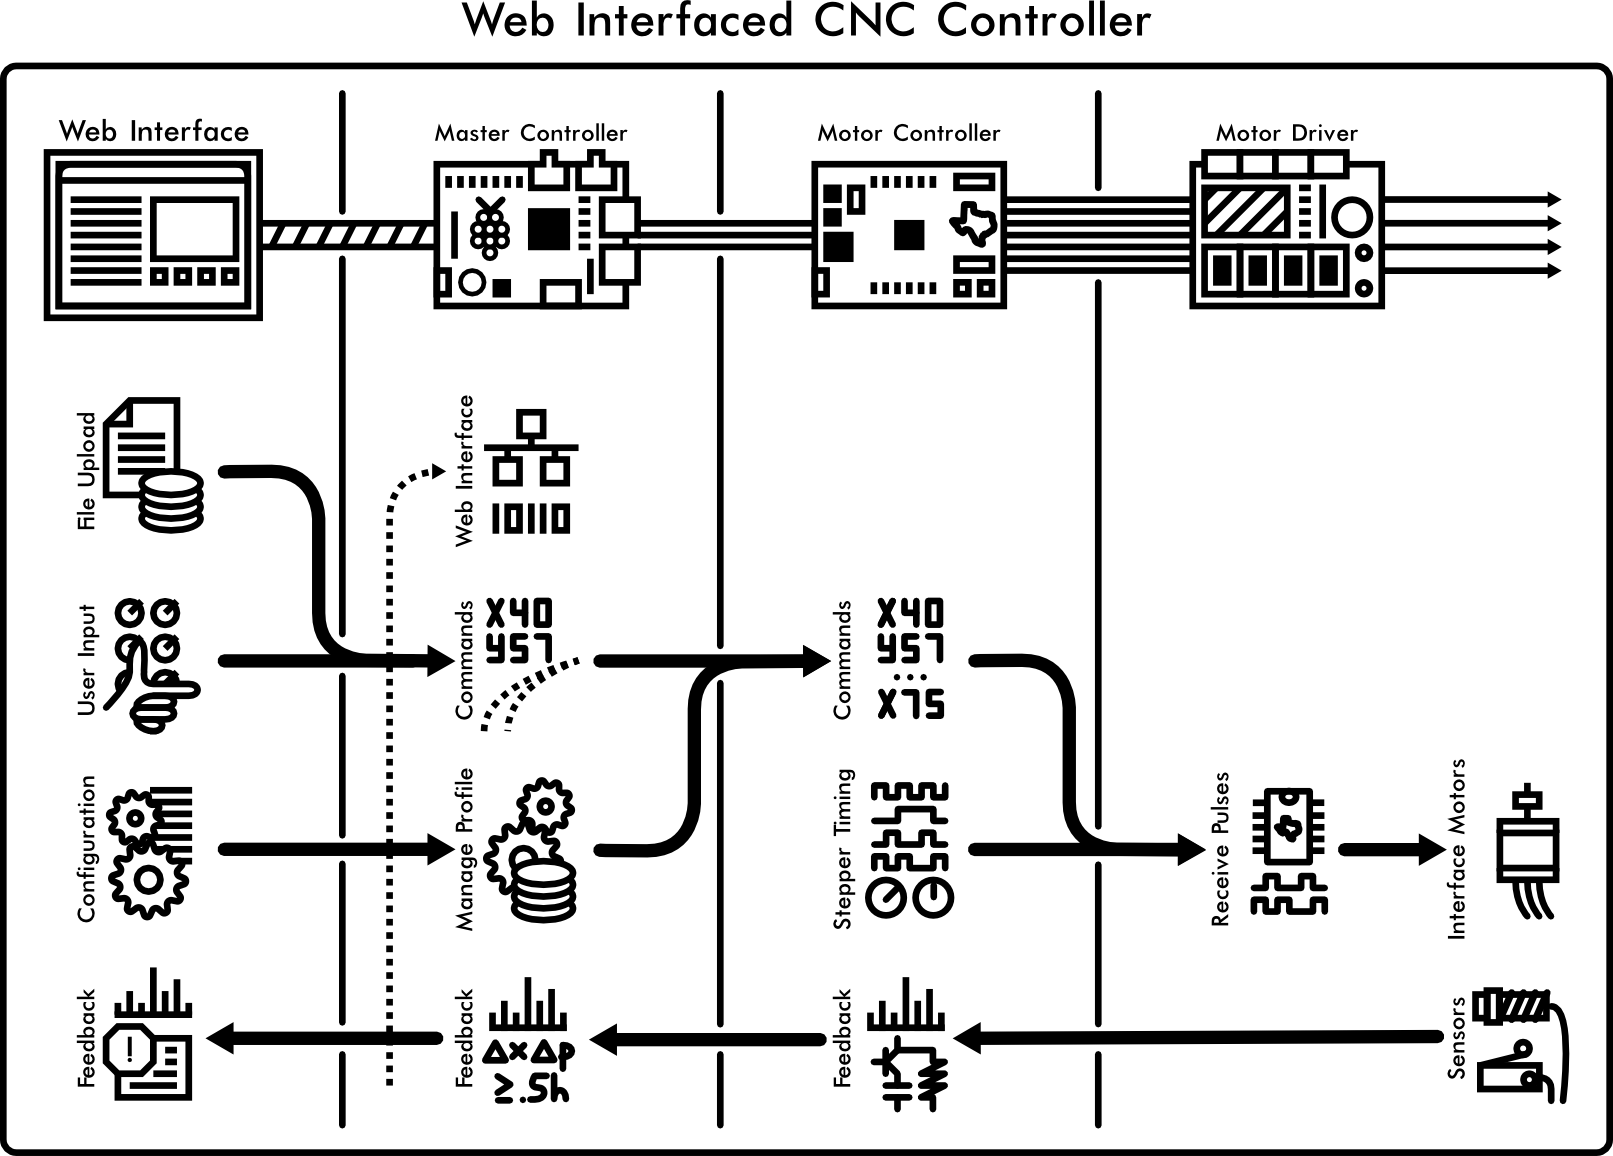
\includegraphics[width=1\textwidth]{architecture.png}
	\caption{System Architecture}
	\label{fig:architecture}
\end{figure} 

\subsection{TCP/IP Interface}
Since sensitive data will not be shared with the device, security is not required, though it is preferred. 
Since plaintext or SSL sockets and SFTP are more difficult to use than the other options, they should not be used since the final product should not require special training. 
HTTPS will be used for its security advantages over HTTP, and ease of use over other methods. 

\begin{table}[h]
\caption{Web Interface Evaluation}
	\label{table:TCPIP}
	\centering
\begin{tabular}{|r|c|c|c|c|c|c|}
\hline
Item              	& Weight & HTTPS  & HTTP       & SFTP        & SSL Socket	& Plaintext\\ \hline
Security       	& 1      & -      & -1         & 0           & 0          	& -1   \\ \hline
Implementation	& 2      & -      & 1          & 0           & -1     		& 1   \\ \hline
Ease of Use       	& 3      & -      & 0          & -1          & -1         	& -1 \\ \hline
Score         	&        & -      & 1          & -3          & -5         	& -2   \\ \hline
Alternative     	&        & Y      & Y          & N           & N       	& N   \\ \hline
\end{tabular}
\end{table}

\subsection{Master Controller}
The \gls{pi} was selected from the following alternitives for its superior hardware, and application notes.
\begin{table}[H]
\caption{Master Controller Evaluation}
	\label{table:MaCEval}
	\centering
\begin{tabular}{|r|c|c|c|c|}
\hline
Item              & Weight & RasPi & Beagle &Arduino \\ \hline
Speed             & 1      & -     & 0                                                     & -1                                                     \\ \hline
Versatility       & 3      & -     & 0                                                     & 0                                                      \\ \hline
GPIO              & 2      & -     & 1                                                     & 1                                                      \\ \hline
Application Notes & 4      & -     & -1                                                    & 0                                                      \\ \hline
Score             &        & -     & -2                                                    & 1                                                      \\ \hline
Alternative       &        & Y     & N                                                    & Y                                                    \\ \hline
\end{tabular}
\end{table}

\subsection{Motor Driver Controller Microcontroller}
Of the following alternatives, the MSP430 was selected for its low cost, adequate timer count, and interrupt capabilities.
\begin{table}[H]
\caption{Motor Controller Evaluation}
	\label{table:uCEval}
	\centering
\begin{tabular}{|r|c|c|c|c|c|}
\hline
Item              	& Weight & MSP430 & ATMega324P & AT90USB1287 & ARM Stellaris \\ \hline
GPIO          	& 1      & -      & 1          & 1           & 1             \\ \hline
SPI         		& 2      & -      & 0          & 0           & 0             \\ \hline
Interrupt			& 3      & -      & 0          & 0           & 0             \\ \hline
Timers        	& 4      & -      & -1         & -1          & 1             \\ \hline
Score         	&        & -      & -3         & -3          & 5             \\ \hline
Alternative     	&        & Y      & N          & N           & Y           \\ \hline
\end{tabular}
\end{table}

\subsection{Motor Drivers}
Of the following alternatives, the DRV8825 was selected for its comparable power capabilities, and superior documentation.
\begin{table}[H]
\caption{Motor Drivers Evaluation}
	\label{table:MCEval}
	\centering
\begin{tabular}{|r|c|c|c|c|}
\hline
Item                   & Weight & DRV8825 & A4988 & TB6560 \\ \hline
Microstepping 	 	& 1      & -       & -1    & -1     \\ \hline
Price                  & 2      & -       & 1     & 1      \\ \hline
Failsafe               & 3      & -       & 1     & -1     \\ \hline                         
Power Output           & 4      & -       & -1    & -1     \\ \hline
Score                  &        & -       & 0     & -6     \\ \hline
Alternative            &        & Y       & Y     & N      \\ \hline
\end{tabular}
\end{table}

\section{Production Schedule}
The \gls{ceenc}'s first plan iteration started as a large reaching product.
After being advise to reduce the scope of the project, the idea for designing and developing just the control interface was decided upon.
At the same time, the main objectives, the \gls{pssc}s, were initially written.
From this point, a plan was formulated.
A \gls{wbs} was designed to break each part of the project into smaller tasks.
Task dependencies were also set up using the \gls{wbs}. 
From here, a \gls{lrc} was designed to assign responsibility of a task to a developer.
The \gls{lrc} and \gls{wbs} were then used to put together an \gls{aon} chart.
This \gls{aon} allowed for a critical path to be determined. 
The critical path is the series of tasks that will take the longest amount of time.
Once dependencies and responsibilities were decided, a realistic schedule could be designed.
This schedule was represented in a Gantt Chart.
This Gantt Chart went through a few iterations of design before the final schedule was set.

Once the schedule was set, the implementation phase of the project started. 
Each member worked on assigned tasks individually or with other members if it was needed.
The project stayed on schedule most of the time.
The progress of the project was tracked in each member's log books, an online tracker, and an \gls{oppm}.
The \gls{oppm} is a document that compiles all the information from the \gls{wbs}, \gls{lrc}, Gantt Chart, and budget onto one page to give to upper management.
Each week, a team meeting was held where updates would be given to make sure that tasks were getting done and to plan the next week's work.
This would also be reflected on the \gls{oppm}.

One recommendation for the next plan would be to include more time for testing. 
Testing was a part of the project that got held up for a variety of reason.
Also, some of the testing time lines were over-ambitious to begin with.

\chapter{Engineering Analysis}

Once design alternatives were evaluated and the anticipated project implementation specifics were chosen, the team set out to professionally implement the design.
This entails carefully designing each of the project's components, including the hardware design, software design, and packaging design.
Thorough design ensured that implementation issues were anticipated and therefore mitigated or avoided.

\section{Packaging Design}
\subsection{Overview}
Packaging for the \gls{ceenc} was constructed primarily from laser cut acrylic, as shown below. 
Laser cutting services were provided by Pokono, for a materials fee and machinery surcharge.
Design of the packaging was completed utilizing InkScape Vector Design Software.
Measurements were taken from the Master, Controller, and Driver boards, then translated into cutouts to support the components.
These cutouts were attatched to the sides of the enclosure, then stabilized by box joints \& machine screws.

\subsection{Design Considerations}
Cooling for the \gls{ceenc} is provided by two 40mm 5v Box Fans attatched to the back of the case.
They push air into the device, which allows egress only through the vents placed directly above the Motor Drivers.
This has the net effect of cooling all components, but with the primary focus on the Motor Drivers.
Interactive LCD components and Port Access was also added to the front and back.

\subsection{Material Selection}
Materials were chosen for both dimesnional stability, and aesthetic properties.
For the prototype unit, selection was limited to materials provided by the manufacturer.
Laser cut acrylic was used for the front and back of the enclosure, to allow for finer detail.
The acrylic chosen was also tinted, to allow for the LCD within the device to be visible when powered, but prevent the rest of the device from showing.
3-Ply laser cut walnut veneer was used for the sides of the enclosure.
This material is both structurally sound, and visually pleasing. 
Costs could be reduced here by choisng a less expensive mediums such as acrylic or cardboard.

\subsection{Cost Analysis}
Enclosure costs are primarily a result of the limited production quantity. 
Material costs for the entirety of the device are well below the \$10.00 mark, but manufacturing fees push the total cost above \$50.00.
Should the \gls{ceenc} be put into production, the total cost for the enclosure is expected to be below \$18.00.
This is calculated based upon laser cutting time cost estimates for large batches, and the existing material cost.
With the present design, full cutting of the enclosure takes between 5 and 10 minutes.
At the standard rate of $50.00 per machine hour, this translates to $8.00 per unit.
Additional costs incurred for processing, shipping, and technician time will not be incurred for larger orders.

\begin{figure}[h]
	\centering
	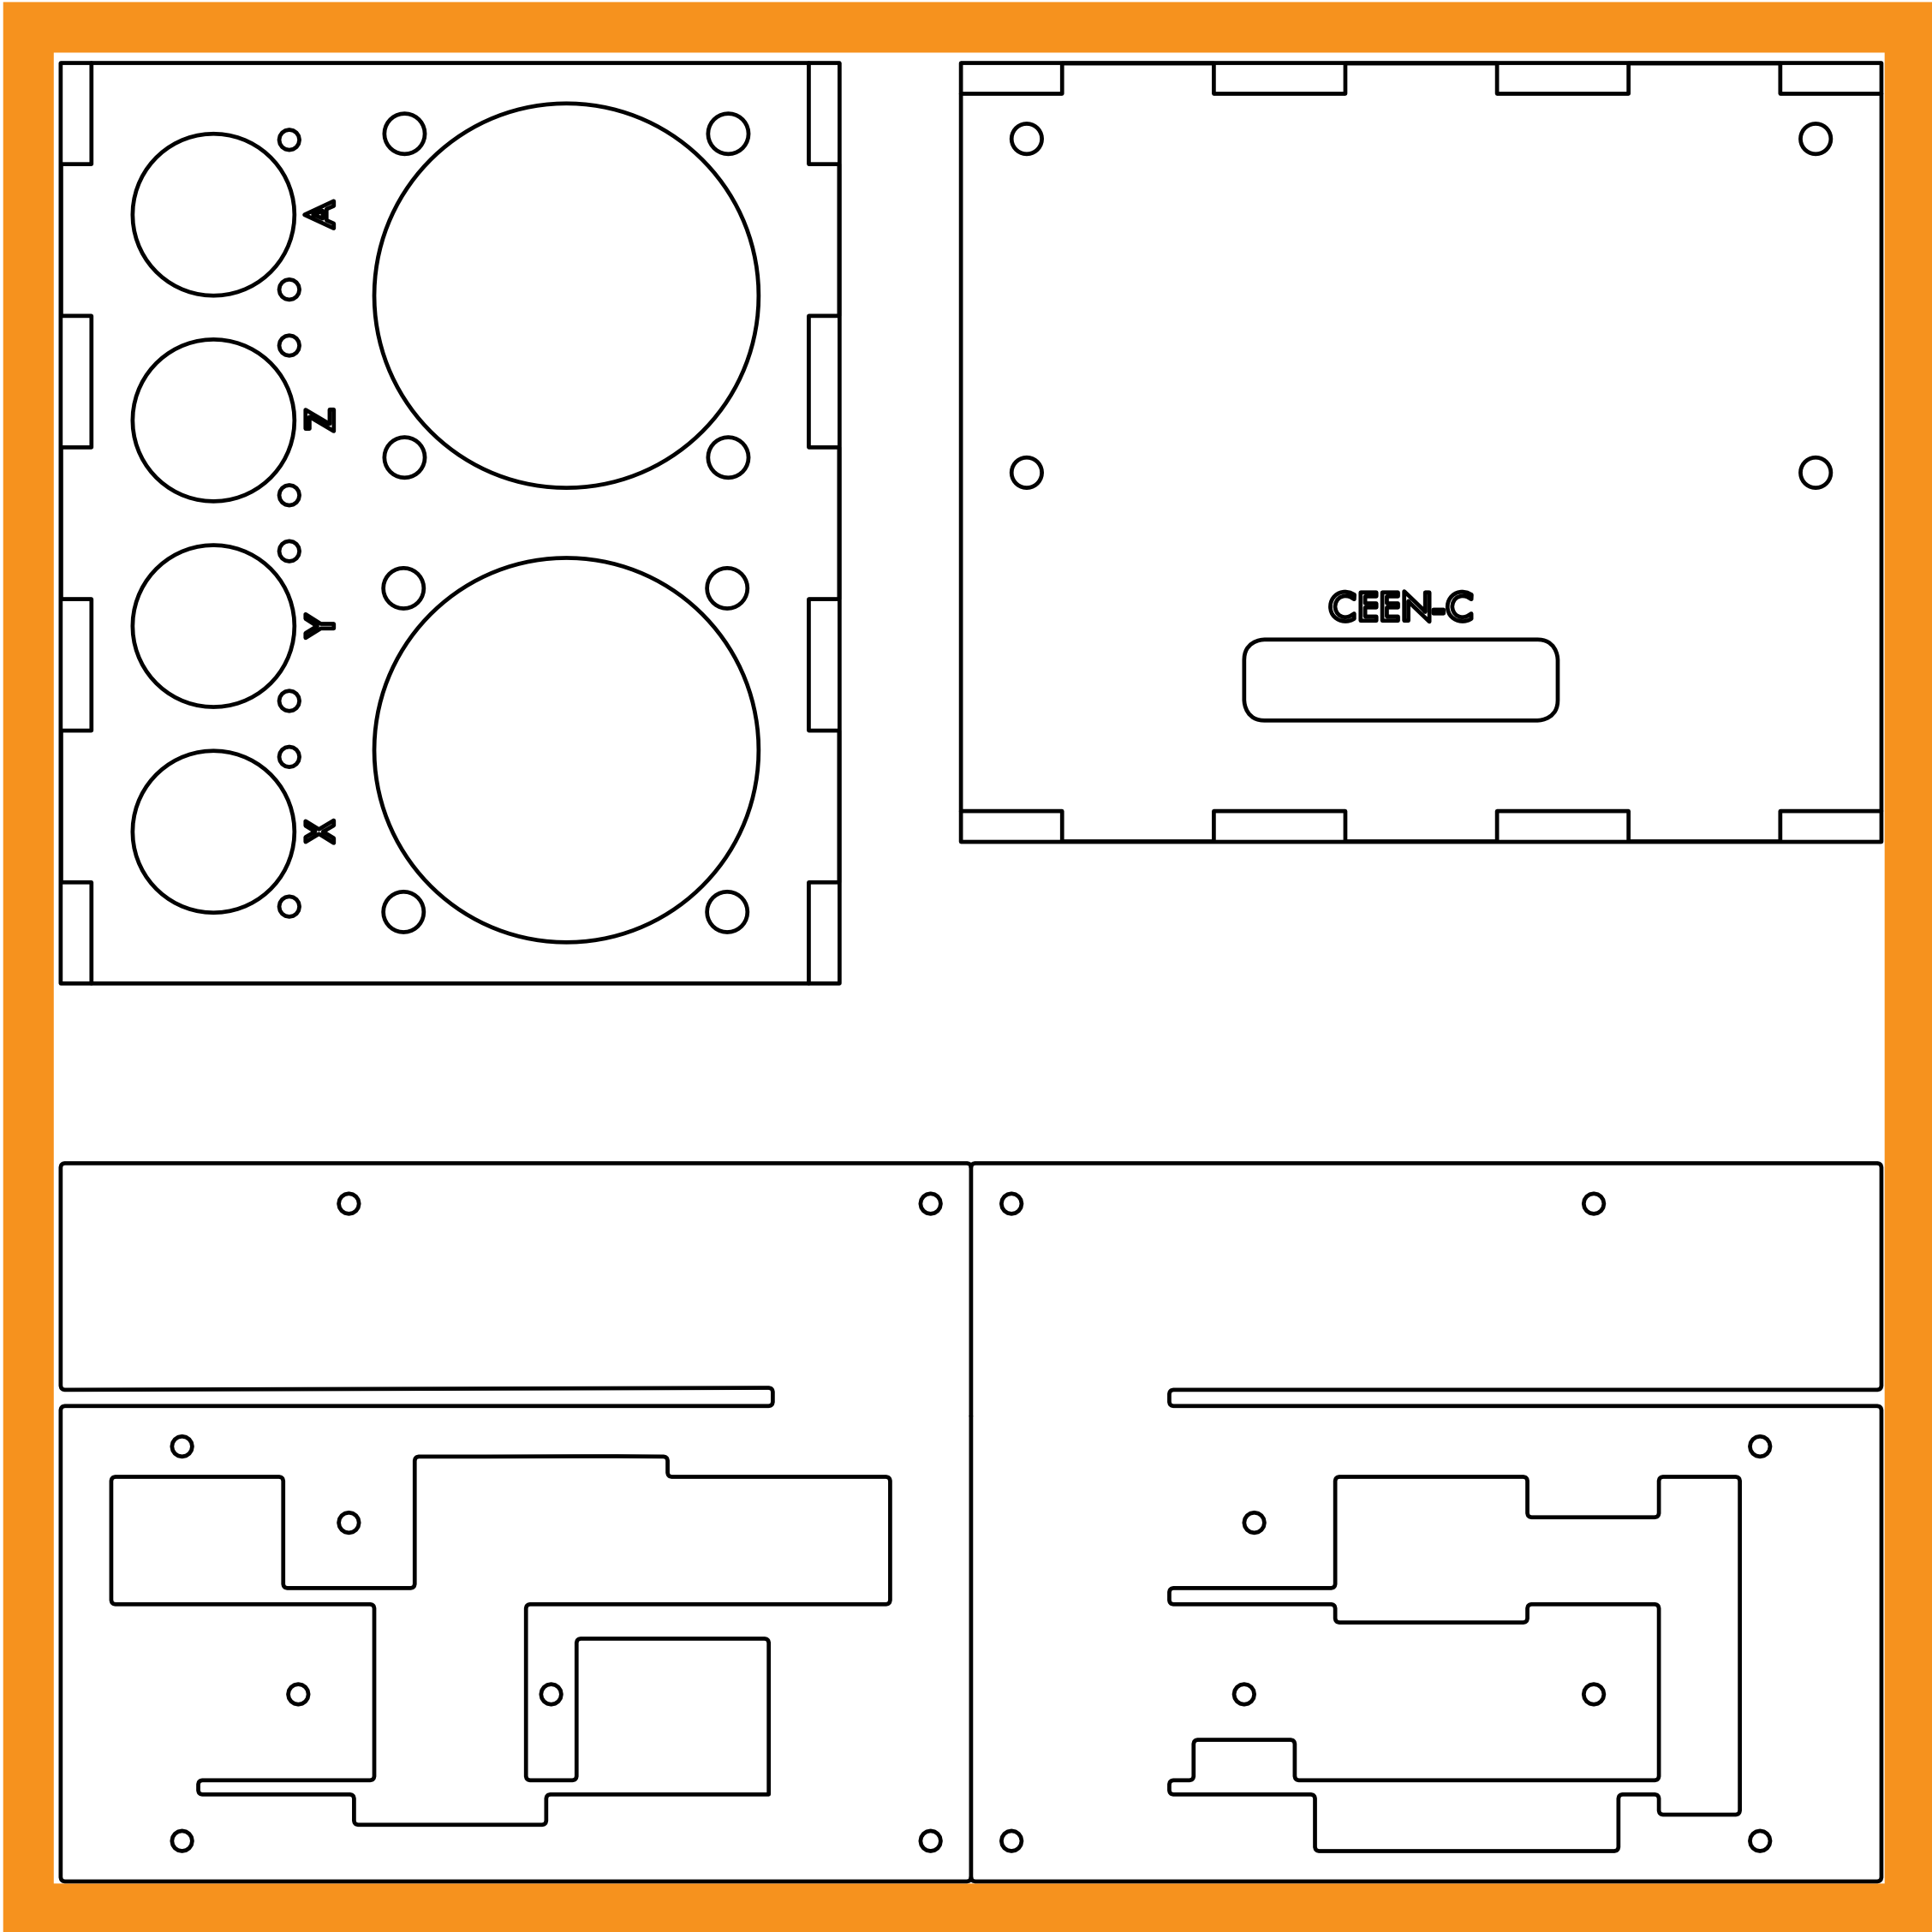
\includegraphics[width=1\textwidth]{packaging-design/front.png}
	\caption{Enclosure Front}
	\label{fig:front}
\end{figure}

\begin{figure}[h]
	\centering
	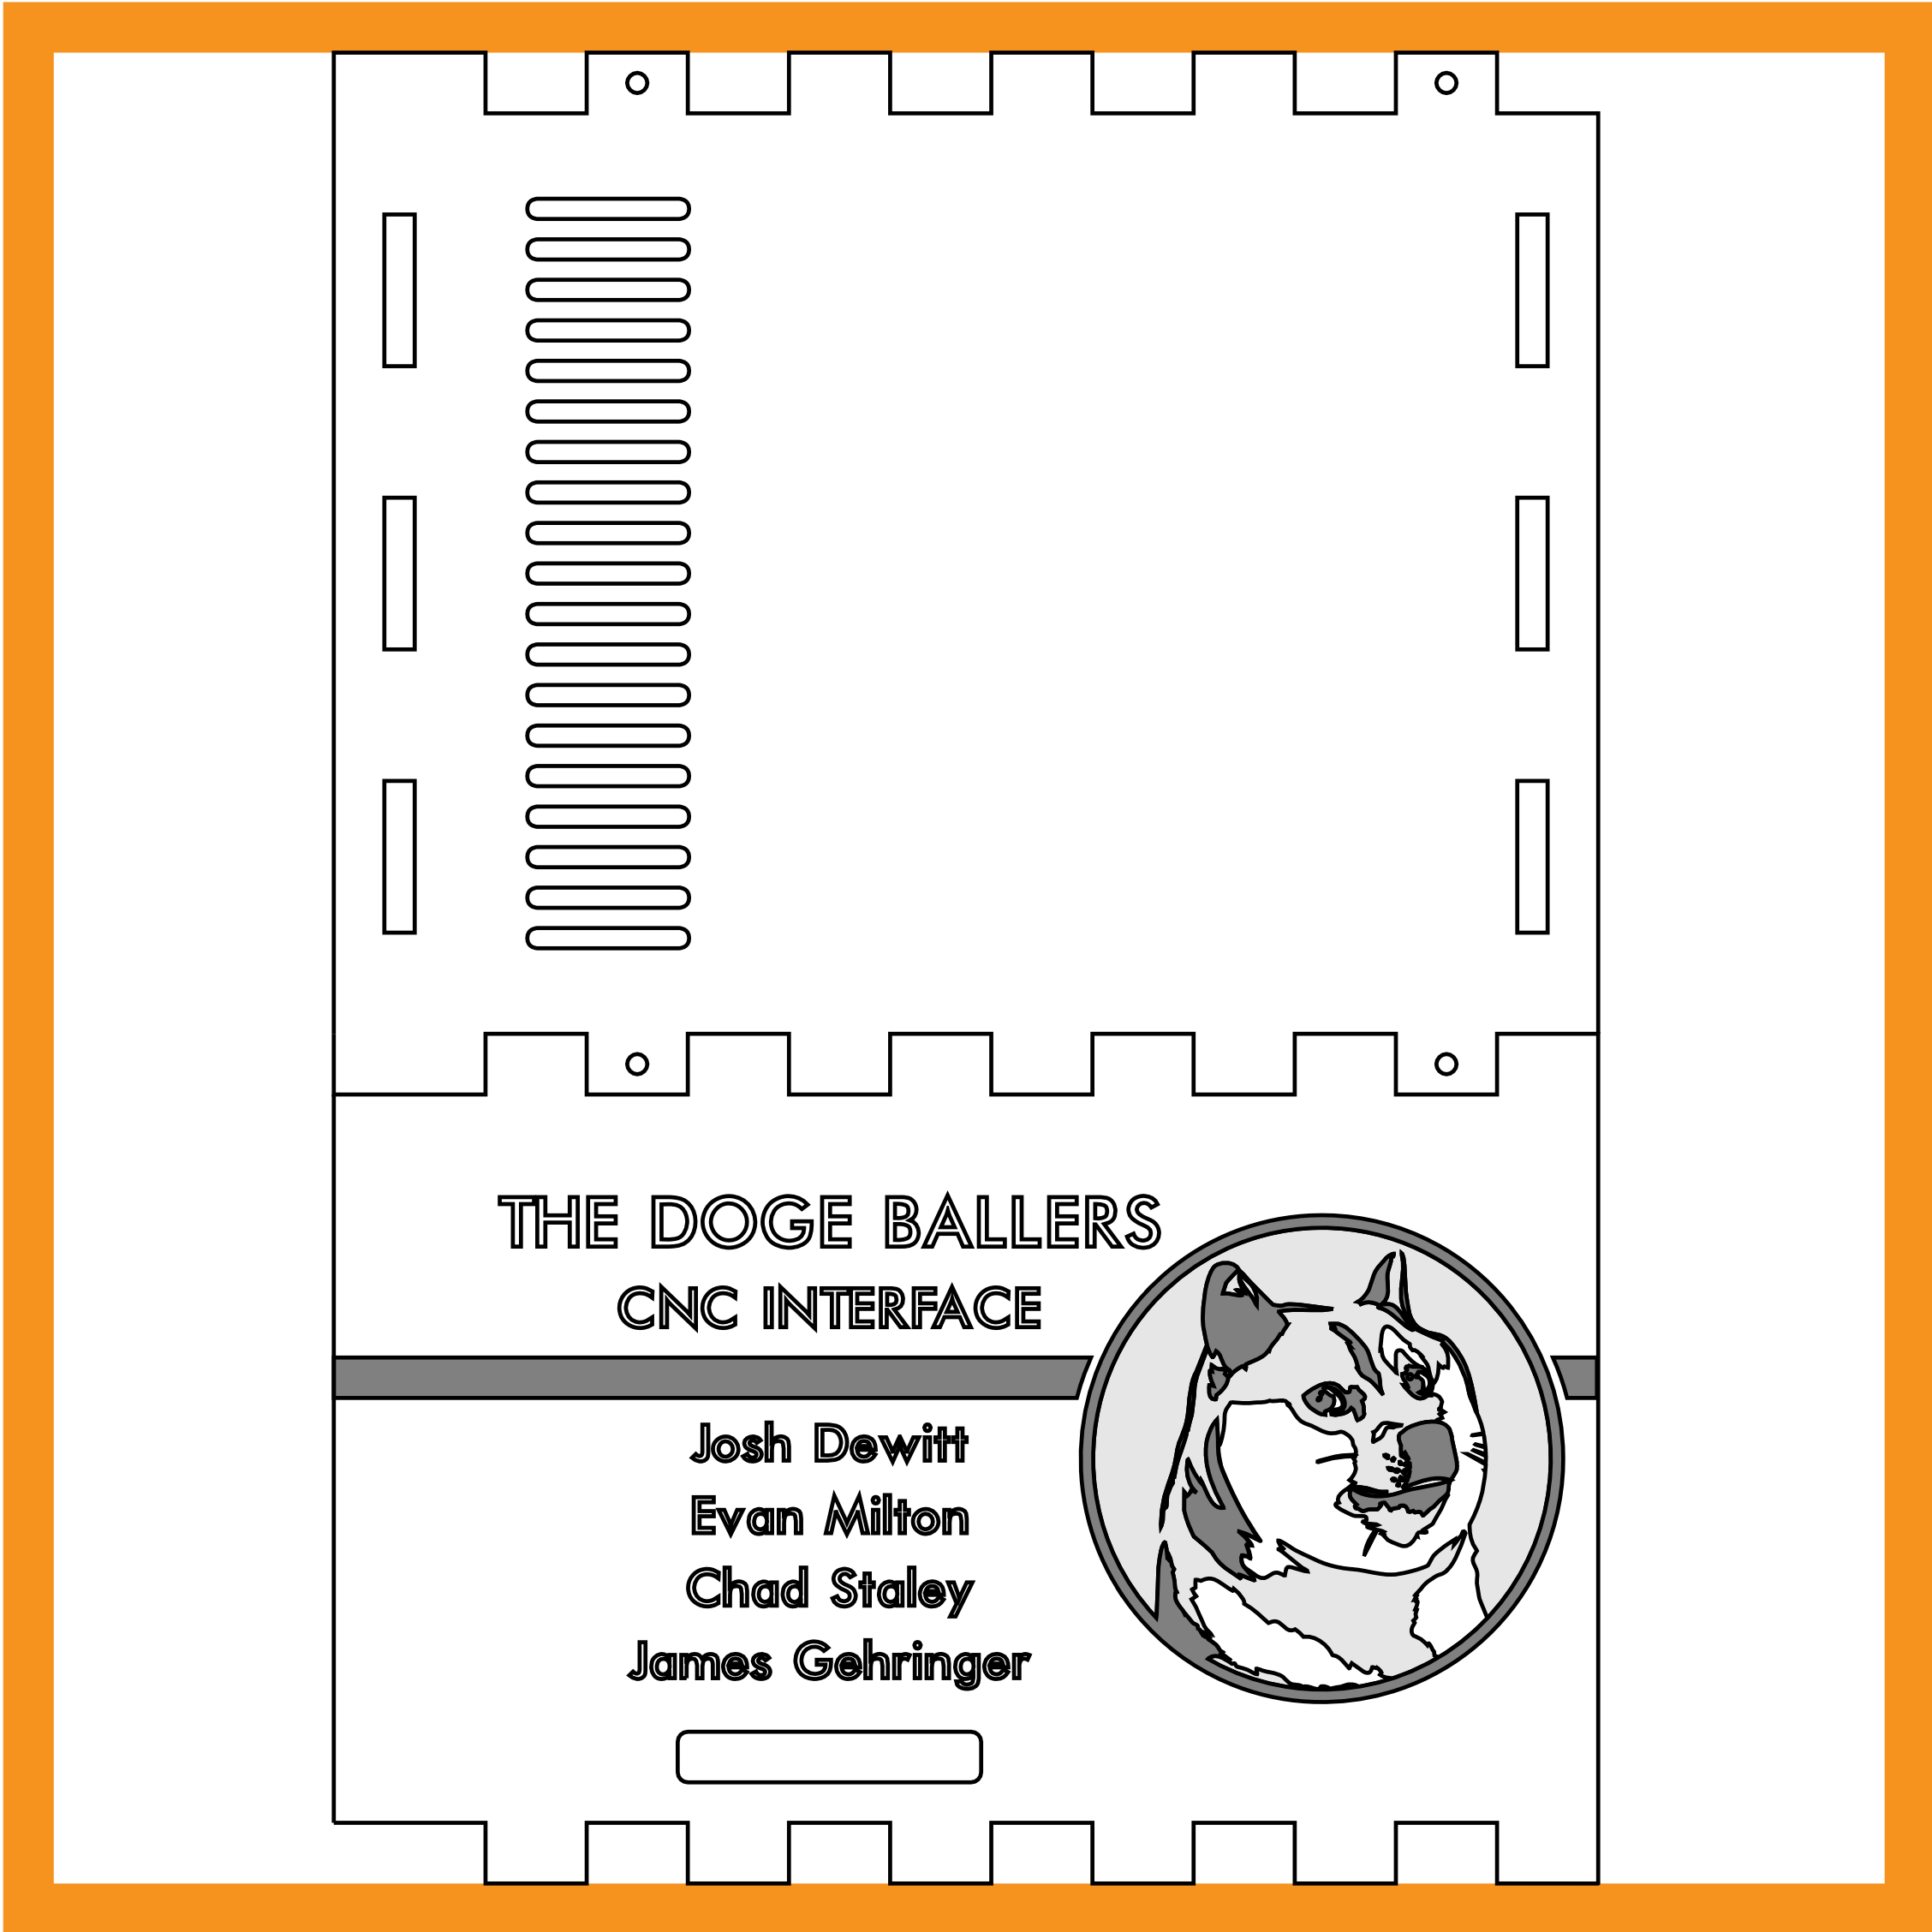
\includegraphics[width=1\textwidth]{packaging-design/side1.png}
	\caption{Enclosure Side Right}
	\label{fig:side1}
\end{figure}

\begin{figure}[h]
	\centering
	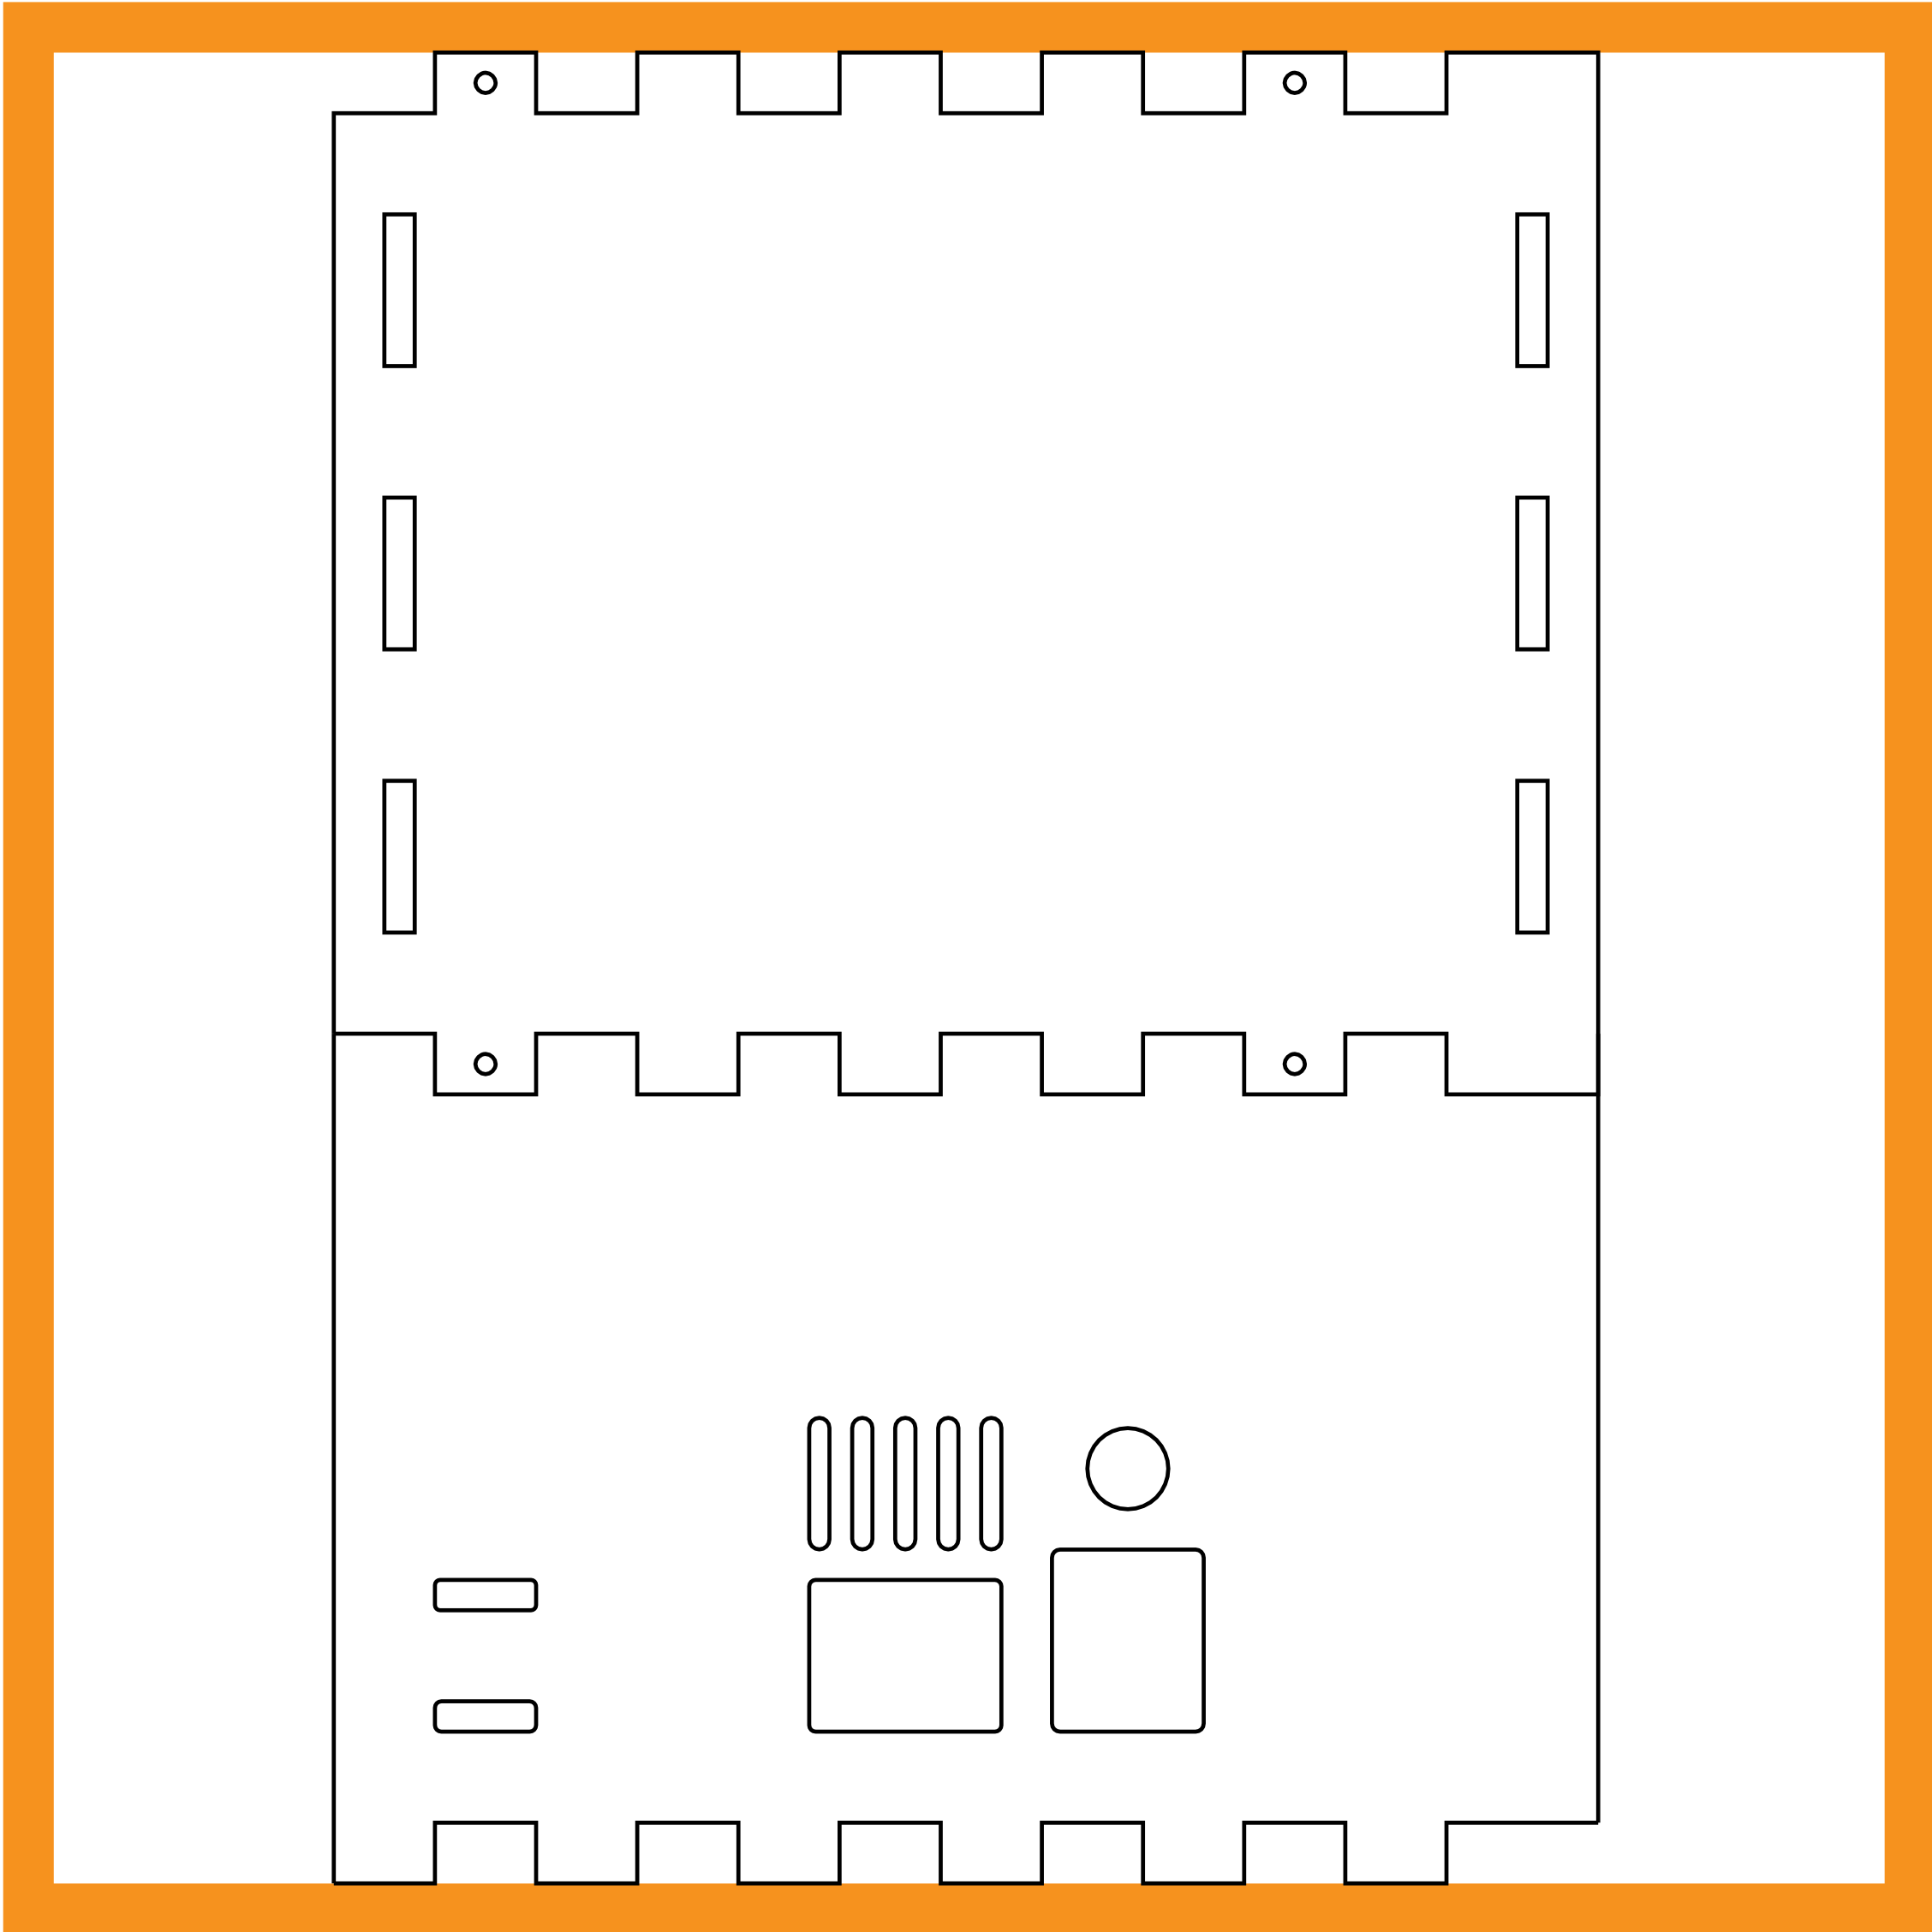
\includegraphics[width=1\textwidth]{packaging-design/side2.png}
	\caption{Enclosure Side Left}
	\label{fig:side2}
\end{figure}

\section{Hardware Design}

\subsection{Introduction}
The \gls{ceenc} consists of three major hardware components, the \gls{pi}, the control board, and the driver board.
The \gls{pi} will handle most of the processing and have a master relationship with the control board.
The control board will be an additional microcontroller that supports the \gls{pi} in timing and motor control functions.
The driver board will receive motor control commands from the control board and execute them using the \gls{ti} DRV8825 motor driver.
The driver board was developed and implemented separately from the control board to allow for early and individual testing.

\subsection{Raspberry Pi}
The \gls{pi} will receive G-code from the web interface over \gls{tcpip} through the Ethernet or USB ports.
The \gls{pi} will send commands to the motor control board microcontroller over a \gls{spi} bus.
The \gls{pi} will send data to a port expander on the control board over an \gls{i2c} connection.
The \gls{pi} will operate in the master mode for the \gls{spi} communication.
The control board will be dependent on the information it receives from the \gls{pi} for motor operation.
\gls{spi} was chosen because it is native on the \gls{pi} and most microcontrollers support it.
The \gls{pi} will be powered from the +5V rail on the control board.

\subsection{Control Board}
The control board will be implemented using the TI C2000 microcontroller.
A microcontroller supports the \gls{pi} so that the stepper motor timers can be run independently from the overhead of an operating system.
The microcontroller will receive commands from the \gls{pi} over a \gls{spi} connection.
The control board will contain an \gls{i2c} port expander that will provide 16 general purpose outputs and is controlled from the \gls{pi}.
The control board will send commands to the driver board over a parallel port connection.
A parallel port was chosen so that the driver board would also be able to interface with the parallel port on some PCs or other \gls{cnc} drivers.
The parallel port also allows for the I/O of the microcontroller to be mapped to the I/O of the motor drivers in a 1-to-1 relationship.
The microcontroller will output step, direction, and enable data for motor control.
It will receive fault and home inputs from the motor driver board.
The step lines must be capable of outputting a 10kHz signal.
A step frequency of 10kHz will be sufficient for \gls{cnc} applications.
The microcontroller uses 4 timers to track of the step count of each motor. 
The control board will have one DC power input.
This power input can range from 14V-36V.
There will be two regulated power supplies on the control board, 5V and 3.3V.
The 5V supply will power the \gls{pi}.
The 3.3V supply will power the microcontroller, the \gls{i2c} port expander, and the opto-isolators on the motor driver board.
The 14V-36V supply will power the motor drivers.

\subsection{Driver Board}
The motor drivers will be implemented using four \gls{ti} DRV8825.
The DRV8825 is a dual stepper/DC motor driver.
Each DRV8825 will receive step and direction commands from the motor control board over a parallel port connection.
The motor driver ICs will step the motors according to the commands from the microcontroller.
The motor driver board contains any necessary pull up/pull down resistors for the motor control signals.



\subsection{Summary}
\newpage
\section{Printed Circuit Board Design}
Standard \gls{pcb} design practices were implemented while designing the two custom \gls{pcb}s for this project.
The \gls{pcb} layout for the motor driver board is show in Figures ~\ref{fig:driver-top-cream} through ~\ref{fig:driver-bottom-copper}.

\subsection{Dimensions}
The \gls{ceenc} is based on the footprint of the \gls{pi}, and as such has stringent design requirements in terms of component layout and dimension.
\gls{gpio} headers must be carried across boards, as well as power connections and mounting points. Board length and width must also match that of the \gls{pi}. 

\subsection{Placement}
These requirements dictate the layout of major components, but leave many of the minor pieces unaccounted for.
After allocating areas for the microcontroller and power supply, major connectors are placed for optimal access to the remaining \gls{gpio}.
Indicator \gls{led}s, and test points are also placed for ease of use during the testing phase, and components are tweaked to provide an aesthetically pleasing, symmetrical layout.
The microcontroller is centrally located, to minimize trace lengths to the outlying components, reducing cross-talk and propagation delays.

\subsection{Power Considerations}
Power supply circuitry is isolated to a single section of the board, so as to limit the potential for interference.
Smoothing capacitors are placed as close as possible to the components for which they will be acting, and indicator \gls{led}s are used to mark active lines.
Larger trace widths are used for power lines as a rule of thumb, but of special consideration are the 10 Amp (instantaneous) lines to feed the driver board.
Positive and zero rails are also routed alongside one another, so as to counteract RF interferences that would otherwise result from the voltage differences.

\section{Software Design}

\subsection{Introduction}
The \gls{cnc} Interface is a project to drive a \gls{cnc} using a simple user interface and no need for installing drivers.
Additionally, the \gls{cnc} Interface will not be plugged into the computer, but will be controlled through the network instead.
The focus of software design for this project was to allow development from day one, not requiring any of the project's hardware to begin.
To achieve this goal, a test-driven development approach was adopted, meaning unit tests that verify project success are created before any application code is written.
This approach has allowed the software development to stay on track and not be pushed off until the end of the project.

\subsection{C2000 Software Design Considerations}
In this project, the \gls{ti} C2000 Piccolo microcontroller was chosen over the cheaper MSP430 because of more device support and available libraries.
The libraries provide an abstraction to the hardware registers allowing faster coding for the device. 

\subsubsection{Memory Model}
\begin{wraptable}{r}{8cm}
	\vspace{-18pt}
	\caption{C2000 Memory Map}
	\label{tab:memory-map}
	\centering
	{\footnotesize
	\begin{tabular}{rl|c|c|}
		\hline\hline
		&& Data Space & Program Space \\ \cline{3-4}
		0x00&0000 & \multicolumn{2}{c|}{M0 Vector RAM} \\ \cline{3-4}
		0x00&0040 & \multicolumn{2}{c|}{Boot Stack, RAM Functions} \\ \cline{3-4}
		0x00&0400 & \multicolumn{2}{c|}{Program Stack} \\ \cline{3-4}
		0x00&0600 & \multicolumn{2}{c|}{Global Variables} \\ \cline{3-4}
		0x00&0800 & Peripheral Frame 0 & Reserved \\ \cline{3-4}
		0x00&0D00 & Interrupt Table & Reserved \\ \cline{3-4}
		0x00&0E00 & Peripheral Frame 0 & Reserved \\ \cline{3-4}
		0x00&2000 & \multicolumn{2}{c|}{Reserved} \\ \cline{3-4}
		0x00&6000 & Peripheral Frame 1 & Reserved \\ \cline{3-4}
		0x00&7000 & Peripheral Frame 2 & Reserved \\ \cline{3-4}
		0x00&8000 & \multicolumn{2}{c|}{L0 SARAM} \\ \cline{3-4}
		0x00&9000 & \multicolumn{2}{c|}{Reserved} \\ \cline{3-4}
		0x3D&7800 & \multicolumn{2}{c|}{User OTP} \\ \cline{3-4}
		0x3D&7C00 & \multicolumn{2}{c|}{Reserved} \\ \cline{3-4}
		0x3F&0000 & \multicolumn{2}{c|}{Flash Program Code, Static Data} \\ \cline{3-4}
		0x3F&7FF6 & \multicolumn{2}{c|}{Flash Program Boot Location} \\ \cline{3-4}
		0x3F&7FF8 & \multicolumn{2}{c|}{128-bit Password} \\ \cline{3-4}
		0x3F&8000 & \multicolumn{2}{c|}{L0 SARAM} \\ \cline{3-4}
		0x3F&9000 & \multicolumn{2}{c|}{Reserved} \\ \cline{3-4}
		0x3F&E000 & \multicolumn{2}{c|}{Boot ROM} \\ \cline{3-4}
		\hline
	\end{tabular}
	}
\end{wraptable}
This slightly more expensive microcontroller has 12\gls{kb} of \gls{ram} and 64\gls{kb} of Flash allowing ample space for the project's code, along with 2\gls{kb} of \gls{otp} and 16\gls{kb} of factory-programmed \gls{rom} containing power-on boot-loading software and standard math-related tables, like sine and cosine waveforms.
Table~\ref{tab:memory-map} shows the C2000's memory map according to the datasheet\cite{piccolo} and the linker command file for the release configuration.
Note that each memory address is two bytes.
An alternate configuration exists that puts all code in \gls{ram}, but this configuration is only used for debugging because it is faster to load a new program into \gls{ram}.
Frequently executed code copied from flash into \gls{ram} at startup to allow power savings and ensure that it is fetched with 0 wait states on interrupt.

\subsubsection{C2000 Peripheral Usage}
The project makes use of the \gls{spi} for communication with the \gls{pi} during normal operation.
\gls{spi} was chosen because of the high-bandwidth achievable, already verified to work with a 1MHz clock using non-ideal wire jumpers.
The \gls{pi} communicates with the C2000 through \gls{uart} at startup for bootloader functions.
\gls{uart} was chosen because the boot \gls{rom} code defaults to interfacing with the \gls{uart} for serial bootloading.
\gls{gpio} pins are used to drive the direction lines for the motors, generate the stepper motor pulse trains, and read the status of the home and emergency stop signals.

\subsubsection{C2000 Code Architecture}
The C2000 code base uses a combination of polling the \gls{spi} communication device and timer-based interrupt-driven code for generating pulse trains to the motors.
A second interrupt is generated whenever the emergency stop line transitions from high-to-low or low-to-high, in which case all motor movement is stopped as quickly as possible.
The pulse train generation is real-time and must execute code as soon as the auto-reloaded timer expires, so polling for \gls{spi} data can be preempted by the timer interrupt.
An alternate design would be to use interrupt priority and allow the timer to interrupt the \gls{spi} interrupt, however a polling scheme is less risky and is easier to code.
Because communication can be interrupted, the \gls{pi} will require the C2000 to echo back sent data to ensure that the entire communication block was received.
Figure~\ref{fig:c2000-main} depicts the polling loop for the C2000 and figure~\ref{fig:c2000-pulse} depicts the interrupt routine for the pulse train generation.

\subsubsection{Raspberry Pi Code Architecture}
The code written for the \gls{pi} is written to read and write to named Linux pipes, or \gls{fifo} files managed by the \gls{os}.
These services are written to constantly run, so running a g-code file requires writing to a pipe, not starting up a program.
The use of pipes allows to better modularize the code base and avoid duplication by factoring out common code into projects.

\subsubsection{Testing and Debugging}
All code for the project is written after unit tests have been created that can be run on any machine using the program make to verify all application logic before implementing on the \gls{pi} or C2000.
The exception is writing to hardware configuration registers which must be changed, programmed, and manually tested for correctness.
Once these low-level configurations are created and verified, they are kept in a stable state in git and will not undergo unnecessary changes.
Code is considered complete when it passes all unit tests, that is, no code is written unless a failing tests proves that it is required.
It follows that new functionality requires that tests are written first, and code is written to make the tests pass.

\subsection{Software Design Narrative}
The code written for this project is intended to be as modular as possible, avoiding duplication of functionality and increasing testability.
The project relies on free software including the Arch distribution of Linux\cite{archlinux} for the \gls{os} on the \gls{pi}, Apache for web hosting from the \gls{pi}, PHP for creating the back-end services that the website makes calls to, JQuery for creating dynamic web pages, and CuTest, a lightweight unit testing framework for C projects.
As shown in figure~\ref{fig:firmware-hierarchy}, the project contains four software modules: the website control, g-code interpreter, \gls{cnc} driver, and the motor scheduler.
The bootloader on the C2000 is programmed into \gls{rom} and is thus not developed or maintained for this project.
Though not used during normal operation, a set of bash scripts grouped together to create a simple way to set up the \gls{pi} was created to be able to quickly set up the \gls{pi} and get ready for development.

\subsubsection{Website Control}
The website control project is written in HTML, CSS, JavaScript, and PHP and is the main interface between the user and the \gls{cnc}.
The website gives the user the ability to upload, delete, and run g-code files and configure the \gls{cnc}'s characteristics, like gearing ration, maximum speed, and maximum acceleration.
The website has been set up, outlined, and approximately 85\% written, with all written code being completely tested.

\subsubsection{g-code Interpreter}
The g-code interpreter project is written in C and is responsible for reading g-code line-by-line and interpreting it into instructions for the C2000 to generate the motor pulse trains.
The g-code interpreter listens to a pipe for g-code commands, which may come from a g-code file or directly from the website when the user is homing the machine, then writes to another pipe that is received by the \gls{cnc} driver.
At startup, the g-code interpreter is responsible for driving the state of the C2000, instructing it to home the \gls{cnc}.
The g-code interpreter relies heavily on mathematic formulas created by the software engineer, so many unit tests have been written to ensure proper functionality.
The g-code interpreter has been outlined, flow-charted, and approximately 90\% written, with all written code being completely tested.

\subsubsection{\gls{cnc} Driver}
The \gls{cnc} driver project is written in C and is responsible for managing communication channels between the \gls{pi} and C2000 through the \gls{spi} and \gls{uart}.
The g-code interpreter does not write to the \gls{spi} or \gls{uart} directly because these actions require root privileges, so this project was created to allow a single, small program to run as root, while the larger, more frequently changing programs are run by regular users.
The \gls{cnc} driver listens to a pipe for commands to send to the C2000 and forwards them through \gls{spi}, verifying that it is received based on the echo back from the C2000.
The \gls{cnc} driver also looks for a special command that indicates that the next bytes will be \gls{ti} hex data and the program should reset the C2000 and bootload the device with new code.
The \gls{cnc} driver has been outlined, flow-charted, and 100\% written and tested.

\subsubsection{Motor Scheduler}
The motor scheduler project is written in C and is responsible for listening for commands from the \gls{pi} and generating the pulse trains to the motors.
The project is based off an algorithm that requires no floating point operations on the C2000 for generating pulses, saving resources and allowing better real-time performance.
The commands are accepted through \gls{spi} and are acknowledged by echoing back the received data, with the command format specified in a C header file shared between the g-code interpreter and this project.
The motor scheduler has been outlined, flow-charted, and approximately 65\% written, with all written code being completely tested.

\subsection{Summary}
The \gls{cnc} Interface's software is currently on-time because of the development approaches involving test-driven development and well thought-out modular software architecture that makes changes simple and low-risk.
The software hierarchy is a modular design that takes advantage of the available features of the Linux \gls{os} for faster development.
To aid in rapid development and implementation all firmware upgrades to any component of the \gls{cnc} Interface can be made remotely.
A user can \gls{ssh} into the \gls{pi} and make changes to the website control, g-code interpreter, or \gls{cnc} driver projects directly and bootload new C2000 code over the \gls{uart}.
The software architecture created for this project is robust and encourages changes in improvements, while mitigating change risks through unit testing.


\section{Design Performance}
The product performs as expected.
All of the objectives were met.
When a mill is combined with a \gls{ceenc}, the mill correctly mills a design in a timely fashion. 
The general purpose outputs work correctly.
The system can drive four stepper motors, one DC motor, and receives input from an emergency stop switch and 4 stepper home inputs.
The g code used to execute commands can be sent over \gls{tcpip}.
The steppers are driven at a frequency range of at least 10kHz within 5\% accuracy.
The whole system can handle a variety of power supplies and draws no more than 10 amps.
The thermal shutdown also is triggered when the system reaches $60^{\circ}C$.
\chapter{Economic Analysis}
%should be societal/global?
\section{Economic Analysis}
The \gls{cnc} is one of few growing hardware based enterprises in the modern technology market.
In allowing manufacturers greater control over the production process, a wider variety of goods can be produced with limited machinery.
This in turn means that fewer capital resources are required in manufacturing, and production centers can be localized.
Consumers will benifit greatly from the "highly flexible, small-scale manufacturing"\cite{3dprintimpact} provided by the \gls{cnc}.

The \gls{ceenc} brings this technology to an even broader audience, in allowing consumers themselves to produce goods from raw materials.
Persons may circumvent the supply chain entirely, by uploading and milling custom objects on the device.\cite{3dprintsave}
For example, in past years obtaining a differential retainer clip for a 1987 Nissan Hardbody Pickup Truck may have involved a trip to the store, and an order from a centralized warehouse.
This measure could be circumvented entirely however, if the store were to provide \gls{cnc} services, and manufacture the item on the spot. 
Distribution can be made even simpler by making it a household device.

Procuring parts from washing machine load couplers to blender bases with the \gls{ceenc} is as simple as uploading a file.
This in turn increases the overal product lifespan.
While this project has been completed on strictly non-profit grounds, the economic implications for the technology as a whole is staggering.

\section{Manufacturability and Cost Analysis}
Component selection for the \gls{ceenc} was centered around ease of diagnosis, repair, and human assembly.
This in turn puts the system as it stands at a disadvantage for mass production, but inhibited the growth of 3214 gray hairs between its 4 designers.
Should the device go into production, components will be selected based on size, cost, and package. 
The DRV8825 breakout boards will be placed directly on the device, and as many through-hole components as possible will be replaced with surface mount equivalents.
The \gls{pi} will also be eliminated from the system, and the entire assembly placed on a single board.

While operational environment concerns were largely ignored for the prototyping of this device, its use in high dust conditions delegates the need for conformal coating on all surfaces.
Potting compound should also be applied to reduce damages incurred from excessive vibration.
Finally, the enclosure should be made to manage airflow in a manner that mitigates the migration of mites into the membrane of its heat sinks.

\section{Bill of Materials}
\subsection{Total Expenditures}
See appendix...
\subsection{Cost Per Unit}
See appendix...
\begin{table}[h]
\centering
\resizebox{0.95\textwidth}{!}{
\begin{tabular}{llllllll}
\hline
\textbf{QTY} & \textbf{Item}                                     & \textbf{Each}    & \textbf{Sum}     & \textbf{Total}    & \textbf{Retailer} & \textbf{Sales Order}  & \textbf{Date}       \\  \hline \hline
\textit{1}   & \textit{Adafruit Order No. 1 Shipping}            & \textit{\$3.99}  & \textit{\$3.99}  & \textit{\$11.94}  & \textit{Adafruit} & \textit{-}            & \textit{10/14/2013} \\
1            & Pi Cobbler                                        & \$7.95           & \$7.95           &                   &                   &                       &                     \\  \hline \hline
\textit{1}   & \textit{Ti Order No. 1 Shipping}                  & \textit{\$0.00}  & \textit{\$0.00}  & \textit{\$96.75}  & \textit{TI Store} & \textit{318260}       & \textit{1/17/2014}  \\
3            & F28027 - C2000 Piccolo LaunchPad                  & \$17.05          & \$51.15          &                   &                   &                       &                     \\
3            & PCB- Actually from OSHPark                        & \$15.20          & \$45.60          &                   &                   &                       &                     \\  \hline \hline
\textit{1}   & \textit{Pololu Order No. 1 Shipping}              & \textit{\$5.95}  & \textit{\$5.95}  & \textit{\$61.75}  & \textit{Pololu}   & \textit{1J149598}     & \textit{2/5/2014}   \\
4            & DRV8825 Stepper Motor Driver Carrier              & \$13.95          & \$55.80          &                   &                   &                       &                     \\  \hline \hline
\textit{1}   & \textit{Digikey Order No. 1 Shipping}             & \textit{\$10.74} & \textit{\$10.74} & \textit{\$76.21}  & \textit{Digikey}  & \textit{38626132}     & \textit{2/5/2014}   \\
4            & CONN DIN 8POS FEMALE SHIELDED                     & \$1.87           & \$7.48           &                   &                   &                       &                     \\
10           & CONN CIRCULAR DIN 8 PIN MALE                      & \$1.40           & \$13.99          &                   &                   &                       &                     \\
25           & OPTOCOUPLER TRANS 5KVRMS 4DIP                     & \$0.33           & \$8.25           &                   &                   &                       &                     \\
3            & DSUB R/A US 25POS SOCKET                          & \$1.35           & \$4.05           &                   &                   &                       &                     \\
4            & CONN D-SUB PLUG 25POS IDC GOLD                    & \$2.64           & \$10.56          &                   &                   &                       &                     \\
2            & CONV DC/DC 7.5W 36VIN 5VOUT                       & \$4.30           & \$8.60           &                   &                   &                       &                     \\
3            & POLYSWITCH RXE SERIES 3.00A HOLD                  & \$0.66           & \$1.98           &                   &                   &                       &                     \\
3            & PTC RESETBL 60V 750MA SMD 2920                    & \$0.72           & \$2.16           &                   &                   &                       &                     \\
4            & TERM BLOCK HDR 2POS R/A 5.08MM                    & \$0.72           & \$2.88           &                   &                   &                       &                     \\
4            & TERM BLOCK PLUG 2POS STR 5.08MM                   & \$0.57           & \$2.28           &                   &                   &                       &                     \\
10           & CONTACT CRIMP 0.5-1.0 TIN                         & \$0.32           & \$3.24           &                   &                   &                       &                     \\  \hline \hline
\textit{1}   & \textit{eBay Order No. 1 Shipping}                & \textit{\$0.00}  & \textit{\$0.00}  & \textit{\$36.37}  & \textit{eBay}     & \textit{Item No.}     & \textit{2/5/2014}   \\
1            & SUPERNIGHT™ 24V 10A 240W Switching                & \$23.39          & \$23.39          &                   &                   & 331060683775          &                     \\
5            & 8 Pin Circular DIN Connector Right Angle Female   & \$1.00           & \$4.99           &                   &                   & 150898188352          &                     \\
1            & Emergency Stop Switch Push Button Mushroom        & \$7.99           & \$7.99           &                   &                   & 300963699529          &                     \\  \hline \hline
\textit{1}   & \textit{Pololu Order No. 2 Shipping}              & \textit{\$5.95}  & \textit{\$5.95}  & \textit{\$49.75}  & \textit{Pololu}   & \textit{1J149598}     & \textit{2/17/2014}  \\
4            & DRV8824 Stepper Motor Driver Carrier              & \$10.95          & \$43.80          &                   &                   &                       &                     \\  \hline \hline
\textit{1}   & \textit{eBay Order No. 2 Shipping}                & \textit{\$3.25}  & \textit{\$3.25}  & \textit{\$34.99}  & \textit{eBay}     & \textit{Item No.}     & \textit{2/17/2014}  \\
4            & 2 PCS OF A HALL EFFECT SENSOR                     & \$5.38           & \$21.50          &                   &                   & 261186753702          &                     \\
50           & OSRAM Orange SMD 0805 LED                         & \$0.08           & \$3.99           &                   &                   & 201002558121          &                     \\
20           & \#22ga. 6 Conductor Stranded Wire 22 awg /6c      & \$0.48           & \$9.50           &                   &                   & 171244693784          &                     \\  \hline \hline
\textit{1}   & \textit{OSH Park Order No. 2 Shipping}            & \textit{\$0.00}  & \textit{\$0.00}  & \textit{\$37.15}  & \textit{OSH}      & \textit{zA3aNUBm}     & \textit{2/27/2014}  \\
3            & Control Board PCB                                 & \$12.38          & \$37.15          &                   &                   &                       &                     \\  \hline \hline
\textit{1}   & \textit{Adafruit Order No. 2 Shipping}            & \textit{\$4.07}  & \textit{\$4.07}  & \textit{\$9.92}   & \textit{Adafruit} & \textit{445212}       & \textit{2/27/2014}  \\
3            & Extended Pi Header                                & \$1.95           & \$5.85           &                   &                   &                       &                     \\  \hline \hline
\textit{1}   & \textit{Digikey Order No. 2 Shipping}             & \textit{\$4.09}  & \textit{\$4.09}  & \textit{\$21.51}  & \textit{Digikey}  & \textit{38863965}     & \textit{2/28/2014}  \\
21           & 2.2uF Ceramic Capacitor                           & \$0.13           & \$2.73           &                   &                   &                       &                     \\
3            & 220Ohm @100MHz Ferrite Bead                       & \$0.12           & \$0.36           &                   &                   &                       &                     \\
3            & 60Ohm @100MHz Ferrite Bead                        & \$0.10           & \$0.30           &                   &                   &                       &                     \\
2            & 5MHz Crystal                                      & \$0.56           & \$1.12           &                   &                   &                       &                     \\
2            & 10MHz Crystal                                     & \$0.56           & \$1.12           &                   &                   &                       &                     \\
2            & 15MHz Crystal                                     & \$0.57           & \$1.14           &                   &                   &                       &                     \\
2            & 20MHz Crystal                                     & \$0.56           & \$1.12           &                   &                   &                       &                     \\
2            & 3.3V Switching Reg                                & \$4.30           & \$8.60           &                   &                   &                       &                     \\
3            & 140mA Resettable Fuse                             & \$0.31           & \$0.93           &                   &                   &                       &                     \\  \hline \hline
\textit{1}   & \textit{Ti Order No. 2}                           & \textit{\$0.00}  & \textit{\$0.00}  & \textit{\$0.00}   & \textit{Ti}       & \textit{2802784}      & \textit{2/28/2014}  \\
1            & TMS320F28027PTT                                   & \$0.00           & \$0.00           &                   &                   &                       &                     \\
1            & TMS320F28027FPTQ                                  & \$0.00           & \$0.00           &                   &                   &                       &                     \\
3            & PCF8575PWRE4                                      & \$0.00           & \$0.00           &                   &                   &                       &                     \\  \hline \hline
\textit{1}   & \textit{eBay Order No. 3 Shipping}                & \textit{\$2.99}  & \textit{\$2.99}  & \textit{\$7.02}   & \textit{eBay}     & \textit{-}            & \textit{2/28/2014}  \\
1            & 200 ct jumpers                                    & \$4.03           & \$4.03           &                   &                   &                       &                     \\  \hline \hline
\textit{1}   & \textit{Pokono Order No. 1 Shipping \& Art Stuff} & \textit{\$11.79} & \textit{\$11.79} & \textit{\$140.44} & \textit{Pokono}   & \textit{140593}       & \textit{3/28/2014}  \\
1            & Making                                            & \$29.30          & \$29.30          &                   &                   &                       &                     \\
1            & Materials                                         & \$13.00          & \$13.00          &                   &                   &                       &                     \\
1            & Rush Fee                                          & \$6.35           & \$6.35           &                   &                   &                       &                     \\
4            & DogeBall Shirts - \$20 each.                      & \$20.00          & \$80.00          &                   &                   &                       &                     \\  \hline \hline
\textit{1}   & \textit{Amazon Order No. 1 Shipping}              & \textit{\$0.00}  & \textit{\$8.38}  & \textit{\$20.71}  & \textit{Amazon}   & \textit{102-5739428}  & \textit{3/28/2014}  \\
1            & 1.6mm drill bit                                   & \$1.83           & \$1.83           &                   &                   &                       &                     \\
1            & M2-0.4 Flat head screw x 100 - 10mm               & \$3.25           & \$3.25           &                   &                   &                       &                     \\
1            & M2-0.4 Pan head screw x 100 - 8mm                 & \$3.30           & \$3.30           &                   &                   &                       &                     \\  \hline \hline
\textit{1}   & \textit{Pololu Order No. 3 Shipping}              & \textit{\$3.95}  & \textit{\$3.95}  & \textit{\$55.70}  & \textit{Pololu}   & \textit{1J95145}      & \textit{4/2/2014}   \\
3            & DRV8834 Stepper Motor Driver Carrier              & \$9.95           & \$29.85          &                   &                   &                       &                     \\
2            & DRV8824 Stepper Motor Driver Carrier              & \$10.95          & \$21.90          &                   &                   &                       &                     \\  \hline \hline
\textit{1}   & \textit{eBay Order No. 4 Shipping}                & \textit{\$2.95}  & \textit{\$2.95}  & \textit{\$21.87}  & \textit{eBay}     & \textit{281070108725} & \textit{4/2/2014}   \\
4            & 4x Metal Wire 40mm CPU Fan Grill                  & \$1.78           & \$7.12           &                   &                   &                       &                     \\
4            & FAN 40mm 40 10mm 5V                               & \$2.95           & \$11.80          &                   &                   &                       &                     \\  \hline \hline
\textbf{}    & \textbf{Total}                                    & \textbf{}        & \textbf{}        & \textbf{\$682.08} & \textbf{}         & \textbf{}             & \textbf{}          
\end{tabular}}
\end{table}

\begin{table}[h]
\centering
\resizebox{0.90\textwidth}{!}{
\begin{tabular}{llll}
\hline 
\textbf{QTY} & \textbf{Motor Driver Board}                          & \textbf{EACH} & \textbf{TOTAL} \\
4            & DRV8824 Stepper Motor Driver Carrier                 & \$6.00        & \$24.00        \\
1            & Driver Board PCB                                     & \$15.20       & \$15.20        \\
4            & Conn DIN 8POS Female Shielded                        & \$1.00        & \$4.00         \\
4            & 100uF Electroylyctic Capacitor SMD 6.5mm             & \$0.24        & \$0.96         \\
14           & PC817 Optocoupler 5KVRMS 4DIP Package                & \$0.06        & \$0.84         \\
2            & 40 Pin DIP SIP IC Sockets Adaptor Solder Type        & \$0.39        & \$0.78         \\
1            & Conn DSUB 25Pos Plug                                 & \$0.73        & \$0.73         \\
1            & Conn DSUB 25Pos Socket                               & \$0.65        & \$0.65         \\
2            & 40 Pin 2.54mm Single Row Female Pin Header           & \$0.24        & \$0.48         \\
1            & LM1117 Low Dropout Voltage Regulator IC SMD          & \$0.40        & \$0.40         \\
1            & Terminal Block Socket 2Pos 5.08mm                    & \$0.30        & \$0.30         \\
1            & Terminal Block Socket 2Pos 5.08mm                    & \$0.30        & \$0.30         \\
12           & Mini Jumper 2.54mm Gold Plated Closed Cover          & \$0.02        & \$0.24         \\
1            & DC Power Jack 2.1mm Barrel-Type PCB Mount            & \$0.16        & \$0.16         \\
15           & 330 Ohm Resistor SMD 0805                            & \$0.01        & \$0.15         \\
15           & 1K Ohm Resistor SMD 0805                             & \$0.01        & \$0.15         \\
2            & Contact Crimp 0.5-1.0 Tin                            & \$0.05        & \$0.10         \\
8            & 100nF Ceramic Capacitor SMD 0805                     & \$0.01        & \$0.08         \\
2            & Orange LED SMD 0805                                  & \$0.02        & \$0.04         \\
1            & Wafer Connector 2.54mm 2 Pins                        & \$0.02        & \$0.02         \\
             &                                                      &               & \$49.58        \\  \hline \hline
\textbf{QTY} & \textbf{Motor Controller Board}                      & \textbf{EACH} & \textbf{TOTAL} \\
1            & Control Board PCB                                    & \$12.38       & \$12.38        \\
1            & Microcontroller TMS320F28027                         & \$6.18        & \$6.18         \\
1            & 5.0V Switching Voltage Regulator                     & \$4.30        & \$4.30         \\
1            & Extended Pi Header                                   & \$1.95        & \$1.95         \\
1            & I2C Bus Expander PCF8575                             & \$1.91        & \$1.91         \\
4            & 100uF Electroylyctic Capacitor SMD 6.5mm             & \$0.24        & \$0.96         \\
1            & Conn DSUB 25Pos Plug                                 & \$0.73        & \$0.73         \\
1            & PTC Resettable 750mA Hold Fuse SMD 2920              & \$0.72        & \$0.72         \\
1            & PTC Resettable 3A Hold Fuse                          & \$0.66        & \$0.66         \\
1            & Conn DSUB 25Pos Socket                               & \$0.65        & \$0.65         \\
1            & LM1117 Low Dropout Voltage Regulator IC SMD          & \$0.40        & \$0.40         \\
1            & 40 Pin 2.54mm Double Row Male Pin Header Right Angle & \$0.39        & \$0.39         \\
7            & 2.2uF Ceramic Capacitor SMD 0805                     & \$0.05        & \$0.35         \\
1            & Terminal Block Socket 2Pos 5.08mm                    & \$0.30        & \$0.30         \\
1            & Terminal Block Socket 2Pos 5.08mm                    & \$0.30        & \$0.30         \\
6            & Orange LED SMD 0805                                  & \$0.02        & \$0.12         \\
8            & 2.2K Ohm Resistor SMD 0805                           & \$0.01        & \$0.08         \\
5            & 330 Ohm Resistor SMD 0805                            & \$0.01        & \$0.05         \\
2            & 470 Ohm Resistor SMD 0805                            & \$0.01        & \$0.02         \\
2            & 4.7K Ohm Resistor SMD 0805                           & \$0.01        & \$0.02         \\
2            & 470 Ohm Resistor SMD 0805                            & \$0.01        & \$0.02         \\
1            & 10K Ohm Resistor SMD 0805                            & \$0.01        & \$0.01         \\
             &                                                      &               & \$32.50        \\  \hline \hline
\textbf{QTY} & \textbf{Master Controller Board}                     & \textbf{EACH} & \textbf{TOTAL} \\
1            & Rasberry Pi Model B 512MB                            & \$35.00       & \$35.00        \\
1            & Enclosure Expenses                                   & \$20.00       & \$20.00        \\
             &                                                      &               & \$55.00        \\  \hline
\end{tabular}}
\end{table}

\chapter{Reliability and Safety Analysis}
The \gls{ceenc} must perform its functions of communicating with the user and a \gls{cnc} accurately and avoid all risks wherever possible to maintain customer satisfaction.
The aim at hobbyists instead of industrial design allows for a less reliable device, as hobbyists enjoy debugging and fixing devices, however the system will not have any unnecessary reliability flaws.
This report contains reliability analysis, safety analysis, and \gls{fmeca} and includes action items to improve the overall reliability of the \gls{ceenc}.
The most critical issues in this design involve the inability to immediately halt the \gls{cnc} at the user's request, as these moving components can harm people and property and require safeguards to mitigate risk. 

\section{Reliability Analysis}
The components determined most likely to fail were analyzed for reliability to determine an expected \gls{mttf} for the entire system.
All components chosen are critical and can be considered a series system, so the overall reliability is $R_s(t)=\prod_{i=1}^4R_i(t)$.
This gives an overall failure rate of $\lambda_s=\sum_{i=1}^n\lambda_i$ and a $\gls{mttf}_s=\frac{1}{\lambda_s}$.
Calculation of individual $\lambda$ values was performed based on the Reliability Prediction of Electronic Equipment handbook, MIL-HDBK-217F\cite{mil217f}.

\subsection{Common Parameters}
All devices chosen were best described by the microcircuit model, so several common parameters were found and are shown in table ~\ref{tab:commonparameters} to avoid unnecessary repetition.
\begin{table}[h]
\caption{Common Parameters \gls{mttf} Summary}
\label{tab:commonparameters}
\centering
\begin{tabular}{|>{\centering}m{1.7cm}|>{\centering}m{3.5cm}|>{\centering}m{1cm}|m{9cm}|}
\hline
	Parameter Name & Description & Value & Comments \\ \hline
	$\pi_E$ & Environment Factor & 2.0 & From table in section 5.10\cite{mil217f} given fixed ground environment, that is, moderately controlled environment, not laboratory setting \\ \hline
	$\pi_Q$ & Quality Factors & 2.0 & From table in section 5.10\cite{mil217f} given commercial-grade device \\ \hline
	$\pi_L$ & Learning Factor & 1.0 & From table in section 5.10\cite{mil217f} given production run of over two years \\ \hline
\end{tabular}
\end{table}

\subsection{TMS320F28027 Texas Instruments Microcontroller}
For a microcontroller, the failure rate is $\lambda_p=(C_1\pi_T+C_2\pi_E)\pi_Q\pi_L$ failures$/10^6=796.72*10^{-3}$ failures$/10^6$ hours based on section 5.1\cite{mil217f} using the parameters chosen in tables ~\ref{tab:commonparameters} and ~\ref{tab:tms320f28027parameters}.
This gives a \gls{mttf} of $\frac{1}{\lambda_p}=\frac{10^6}{796.72*10^{-3}}=1.255*10^6$ hours $=143$ years for this component.
\begin{table}[h]
\caption{TMS320F28027 \gls{mttf} Summary}
\label{tab:tms320f28027parameters}
\centering
\begin{tabular}{|>{\centering}m{1.7cm}|>{\centering}m{3.5cm}|>{\centering}m{1cm}|m{9cm}|}
\hline
	Parameter Name & Description & Value & Comments \\ \hline
	$C_1$ & Die Complexity Failure Rate & .56 & From table in section 5.1\cite{mil217f} given 32-bit RISC MOS microcontroller \\ \hline
	$\pi_T$ & Temperature Factor & .646 & $0.1*exp\left(\frac{-E_a}{8.617*10^{-5}}\left(\frac{1}{T_J+273}-\frac{1}{298}\right)\right)$ from section 5.8\cite{mil217f} \\ \hline
	$E_a$ & Effective Activation Energy & .42 & From table in section 5.8\cite{mil217f} given MOS device and $T_J$ \\ \hline
	$T_J$ & Worst Case Junction Temperature & 63.379 & $T_C+\theta_{JC}P$ from section 5.11\cite{mil217f} \\ \hline
	$T_C$ & Case Temperature & 60 & From the \gls{pssc} \\ \hline
	$\theta_{JC}$ & Junction to Case Thermal Resistance & 12.8 & From the datasheet\cite{picollo} \\ \hline
	$P$ & Device Power Dissipation & .264 & From the datasheet\cite{picollo} \\ \hline
	$C_2$ & Package Failure Rate & .0183 & From table in section 5.9\cite{mil217f} given hermetic \gls{smt} device with 48 pins, linear approximation since values are only given for 40 and 64 pins \\ \hline
\end{tabular}
\end{table}

\subsection{OKI-78SR Series 5V Switching Regulator}
For a monolithic MOS device, the failure rate is $\lambda_p=(C_1\pi_T+C_2\pi_E)\pi_Q\pi_L$ failures$/10^6=771*10^{-3}$ failures$/10^6$ hours based on section 5.1\cite{mil217f} using the parameters chosen in tables ~\ref{tab:commonparameters} and ~\ref{tab:oki78srparameters}.
This gives a \gls{mttf} of $\frac{1}{\lambda_p}=\frac{10^6}{771*10^{-3}}=1.297*10^6$ hours $=148$ years for this component.
\begin{table}[h]
\caption{OKI-78SR \gls{mttf} Summary}
\label{tab:oki78srparameters}
\centering
\begin{tabular}{|>{\centering}m{1.7cm}|>{\centering}m{3.5cm}|>{\centering}m{1cm}|m{9cm}|}
\hline
	Parameter Name & Description & Value & Comments \\ \hline
	$C_1$ & Die Complexity Failure Rate & .020 & 101 to 1000 transistor MOS digital device from section 5.1\cite{mil217f} and the datasheet\cite{oki78sr} \\ \hline
	$\pi_T$ & Temperature Factor & 19.18 & $0.1*exp\left(\frac{-E_a}{8.617*10^{-5}}\left(\frac{1}{T_J+273}-\frac{1}{298}\right)\right)$ from section 5.8\cite{mil217f} \\ \hline
	$E_a$ & Effective Activation Energy & .84 & From table in section 5.8\cite{mil217f} given a MOS device and $T_J$  \\ \hline
	$T_J$ & Worst Case Junction Temperature & 82.05 & $T_C+\theta_{JC}P$ from section 5.11\cite{mil217f} \\ \hline
	$T_C$ & Case Temperature & 70 & Assuming a $10^{\circ}C$ temperature increase from the \gls{cpu} temperature specified in the \gls{pssc} \\ \hline
	$\theta_{JC}$ & Junction to Case Thermal Resistance & 13 & From the datasheet \\ \hline
	$P$ & Device Power Dissipation & .927 & Output voltage of 5V, maximum load current of 1.5A with a minimum efficiency of 89\% from the datasheet\cite{oki78sr} \\ \hline
	$C_2$ & Package Failure Rate & .00092 & From table in section 5.9\cite{mil217f} given hermetic package with 3 pins \\ \hline
\end{tabular}
\end{table}

\subsection{LM1117 Texas Instruments Linear Regulator}
For a monolithic bipolar device, the failure rate is $\lambda_p=(C_1\pi_T+C_2\pi_E)\pi_Q\pi_L$ failures$/10^6=71.87$ failures$/10^6$ hours based on section 5.1\cite{mil217f} using the parameters chosen in tables ~\ref{tab:commonparameters} and ~\ref{tab:lm1117parameters}.
This gives a \gls{mttf} of $\frac{1}{\lambda_p}=\frac{10^6}{71.87}=13.914*10^3$ hours $=1.587$ years for this component.
\begin{table}[h]
\caption{LM1117 \gls{mttf} Summary}
\label{tab:lm1117parameters}
\centering
\begin{tabular}{|>{\centering}m{1.7cm}|>{\centering}m{3.5cm}|>{\centering}m{1cm}|m{9cm}|}
\hline
	Parameter Name & Description & Value & Comments \\ \hline
	$C_1$ & Die Complexity Failure Rate & .010 & 1 to 100 transistor bipolar linear device from section 5.1\cite{mil217f} and the datasheet\cite{lm1117}, assuming 30 transistors per op amp and 5 transistors per current source \\ \hline
	$\pi_T$ & Temperature Factor & 3593 & $0.1*exp\left(\frac{-E_a}{8.617*10^{-5}}\left(\frac{1}{T_J+273}-\frac{1}{298}\right)\right)$ from section 5.8\cite{mil217f} \\ \hline
	$E_a$ & Effective Activation Energy & 2.0 & From table in section 5.8\cite{mil217f} given a abipolar device and $T_J$  \\ \hline
	$T_J$ & Worst Case Junction Temperature & 71.38 & $T_C+\theta_{JC}P$ from section 5.11\cite{mil217f} \\ \hline
	$T_C$ & Case Temperature & 65 & Assuming a $5^{\circ}C$ temperature increase from the \gls{cpu} temperature specified in the \gls{pssc} \\ \hline
	$\theta_{JC}$ & Junction to Case Thermal Resistance & 15 & From the datasheet\cite{lm1117} \\ \hline
	$P$ & Device Power Dissipation & .425 & Maximum input voltage of 5V, output voltage of 3.3V, maximum current of 250mA \\ \hline
	$C_2$ & Package Failure Rate & .0013 & From table in section 5.9\cite{mil217f} given hermetic package with 4 pins \\ \hline
\end{tabular}
\end{table}

\subsection{Reliability Analysis Results}
With the three components analyzed, $\lambda_s=796.72*10^{-3}+771*10^{-3}+71.87=73.438$ failures$/10^6$ years, and a \gls{mttf} of $\frac{10^6}{73.438}=13617$ hours $=1.55$ years for the system.
Because the system is aimed at hobbyists, the system need not last for 20 years, but an overall \gls{mttf} of 1.55 years is inadequate.
Initially the 3.3V linear regulator was used for price and simplicity, but it is clearly a liability in the system and should be replaced with a switching regulator like the 5V regulator.
This switching regulator would have a $\lambda$ value less than the 5V regulator component because it would be at a lower temperature and consume less power, giving an overall \gls{mttf} of at least 48.78 years.

The most notable improvement in reliability came from the \gls{pssc} stating a maximum \gls{cpu} temperature of $60^{\circ}C$, which reduced the temperature coefficients in the system in the worst case analysis.
The system will not normally be at $60^{\circ}C$, only in extreme cases.
However, the system would be adequately reliable for hobbyists even if operating at such high temperatures continuously, so long as the linear 3.3V regulator is replaced with a switching regulator.

\section{Safety Analysis}
\gls{ieee} standards were used to guide the safety analysis to understand the risks posed by the \gls{ceenc} project.
Safety Analysis Results were based on the analysis of \gls{ieee} standard C95.1\cite{ieeec951}, \gls{ieee} \gls{nesc}\cite{ieeenesc}, and the moving components that will be attached to the system by the end user. 

\subsection{IEEE C95.1 Radio Frequency Analysis}
\gls{ieee} Standard C95.1\cite{ieeec951} uses the \gls{sar} of the human body relating to radio frequencies of 3kHz to 300GHz, which applies to the wireless component of the project.
The project has a \gls{rf} communication component of standard 802.11b/g/n WiFi via a miniature WiFi USB Module, operating in the 2.4GHz range.
The system may have \gls{rf} noise generated by digital switching components, however their power in the 3kHz to 300GHz range will be orders of magnitude less than the WiFi, so they will be ignored for this analysis.
The system is aimed at hobbyists, so the end user will have an uncontrolled environment, meaning that the \gls{mpe} is $10\frac{W}{m^2}$ according to Table 9 in C95.1 chapter 4\cite{ieeec951}.

The WiFi module has a maximum \gls{rf} output power of $17dBm$, which can be re-written as $1mW*10^{\frac{17}{10}}=50.11mW$.
The volume of a sphere is given by $\frac{4}{3}\pi r^2$, so solving the following equation will give the safe radius that a person could regularly be by the device: $\frac{50.11mW}{\frac{4}{3}\pi r^2}=10\frac{W}{m^2}$.
Simple algebra produces a safe distance of $6.13cm$ from the WiFi module, which is a reasonable distance seeing that this device will not be touched by the consumer, only controlled remotely on a regular basis. 
If the user wishes to move the module, they should issue the shutdown command remotely, which powers down the WiFi module, then disconnect the power and move the device to the new desired location.

\subsection{National Electrical Safety Code Analysis}
\gls{ieee}'s \gls{nesc}\cite{ieeenesc} discusses the safety of installing, operating, and maintenance of electric power for all types of building wiring, including residential.
The main safety concern regarding the \gls{nesc} for the \gls{ceenc} is the connection between wall power and the system that the user purchases separate of the system.
Since this select cannot be directly controlled, the system will be shipped with guidelines on picking a safe power supply for use with the system.
Because the system will be connecting to a power supply of up to 36V, the system uses an industry-standard connection jack that does not expose the voltage line to the user.
Additionally, all packaging in the system will be made of non-conductive materials, and any exposed metal components will be grounded to avoid the risk of electrical shock\cite{ieeenesc}.

\subsection{Moving Parts Analysis}
The \gls{ceenc} does not include the actual motor or work equipment, so the project cannot enforce that the user select a safe work environment for their \gls{cnc}.
The system will be shipped with a large emergency stop button that will stop all motors immediately when pressed.
Software, to be run whenever the system is moved, will be available that prompts the user to press the emergency button and verify that the emergency stop signal was received.
To mitigate the risk of user selection of the work area, the system will be shipped with guidelines on creating a safe work environment for their \gls{cnc}.
These guidelines will include recommendations to have the ability to enclose the work area to avoid physical access to the work area while running the system.
A physical barrier would also help protect against release of parts from the work area during any type of milling procedure.

\subsection{Safety Analysis Results}
The analysis has created the following Safety Requirements that the system must abide by:
\begin{itemize}
	\item Include documentation on safe operating practices for running the \gls{ceenc}.
	\item Include documentation on \gls{rf} emissions from the \gls{ceenc}.
	\item Include guidelines for selecting an appropriate power supply to use with the \gls{ceenc}.
	\item Include safety recommendations when creating a work area to connect to the \gls{ceenc}.
	\item Include an emergency stop button that can be placed near the work area for easy access.
	\item Include a system test that ensures that the emergency stop button is connected and works correctly.
\end{itemize}

\section{Failure Mode, Effects, and Criticality Analysis}
The first step for \gls{fmeca} analysis is to break down the schematic into functional blocks. 
See Appendix~\ref{chap:schematic-breakdown} for the detailed contents of each of the four main functional blocks of the circuit.
Figure~\ref{fig:power-block} depicts the voltage regulation circuitry for the system.
Figure~\ref{fig:connectors-block} depicts the off-board data connectors to the \gls{pi} and the the General Purpose Outputs described in the \gls{pssc}.
Figure~\ref{fig:uc-block} depicts the main \gls{ti} microcontroller on the control board.
Figure~\ref{fig:crystal-block} depicts the crystal used to generate the system clock.

For this analysis, only one of the criticality levels, Catastrophic is retained from the Standard Practice for System Safety\cite{mil882d}.
The reason for this is that life-threatening personal injury is still as important, but all other components of a hobbyist's \gls{cnc}, including motors and frame, will not be valued over \$2000.
Analysis of the possible failures modes of each block, effects, criticality, and suggested actions are shown in table~\ref{tab:fmeca}.

\begin{table}[h]
\caption{Criticality Severity Categories}
\label{tab:criticality}
\centering
\begin{tabular}{|>{\centering}m{2cm}|>{\centering}m{2cm}|>{\centering}m{2cm}|m{9cm}|}
\hline
	Criticality Name & Max $\lambda$ & Minimum \gls{mttf} (y) & Criteria \\ \hline
	Catastrophic & $10^-9$ & 114,080 & Could result in death, permanent total disability, or irreversible severe environmental damage that violates law or regulation, or loss greater than \$2000. \\ \hline
	Critical & $5.70*10^{-6}$ & 20 & Entire \gls{ceenc} requires replacement or loss greater than \$100 but less than \$2000. \\ \hline
	Marginal & $1.14*10^{-5}$ & 10 & Soldered component in system requires replacement or loss greater than \$20 but less than \$100. \\ \hline
	Negligible & $1.14*10^{-4}$ & 1 & Non-soldered component requires replacement or loss less than \$20. \\ \hline
\end{tabular}
\end{table}

\section{Recommendations and Actions Taken}
This report thoroughly analyzed the reliability, safety, and criticality of failures in the \gls{cnc} interface and has created several action items to improve the system.
Reliability analysis discourages the user of a linear 3.3V regulator at high temperatures, so the design will be changed to include a switching 3.3V regulator.
Safety analysis deemed that the largest risks lie with the end user setting up their own \gls{cnc} work area, so the system will ship with safety instructions and guidelines to avoid any personal or equipment loss.
\gls{fmeca} analysis showed that the system should be shipped with instructions on how to replace the most likely to fail components, including automating firmware upgrades to ensure the bugs in software are resolved as quickly as possible.
\gls{fmeca} analysis also showed that use of the \gls{ti} TMS320F28027 microcontroller's bootloader for firmware upgrades would allow the system to remain untouched to perform software upgrades, decreasing risk during disassembly for programming with \gls{jtag}.
Several system tests were created to increase safety and reliability, including system tests for the emergency stop to be run whenever the system is moved and tests of the \gls{ti} microcontroller's crystal accuracy using UTC fetched over from the Internet.

\chapter{Social, Political, and Environmental Impact}

\chapter{Individual Contributions}
\chapter{Conclusion}

\begin{appendices}
	\chapter{Firmware Flowchart}

\begin{figure}[!ht]
	\centering
	\begin{minipage}{.45\textwidth}
		\centering
		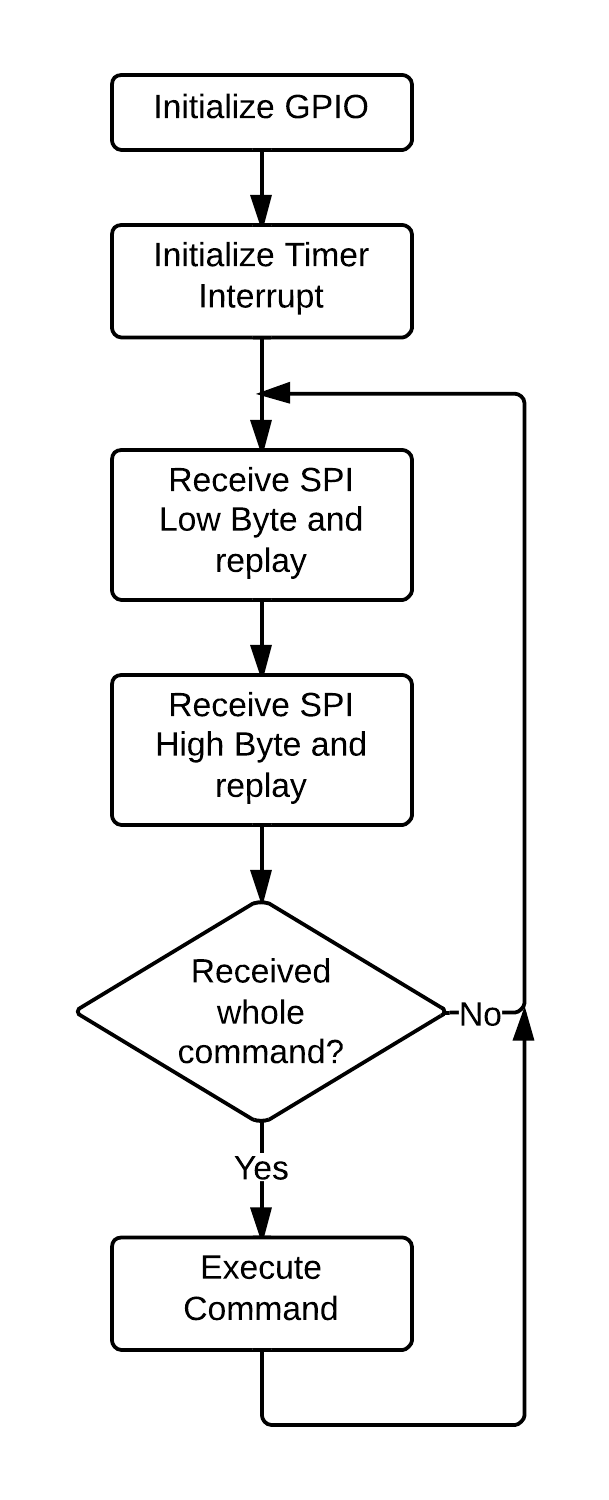
\includegraphics[width=.75\textwidth]{software-design/c2000-main.png}
		\caption{C2000 Main Program}
		\label{fig:c2000-main}
	\end{minipage}
	\begin{minipage}{.45\textwidth}
		\centering
		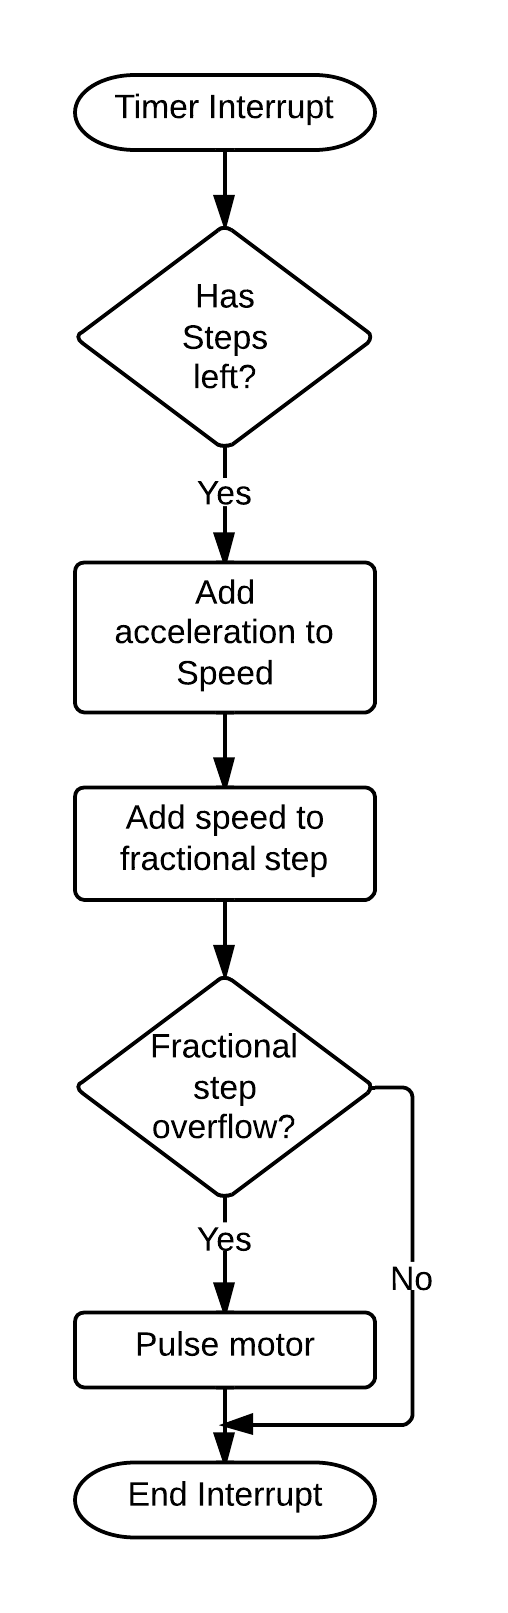
\includegraphics[width=.75\textwidth]{software-design/c2000-pulse.png}
		\caption{C2000 Pulse Generation}
		\label{fig:c2000-pulse}
	\end{minipage}
\end{figure}
	\chapter{Firmware Hierarchy}

\begin{figure}[!ht]
	\centering
	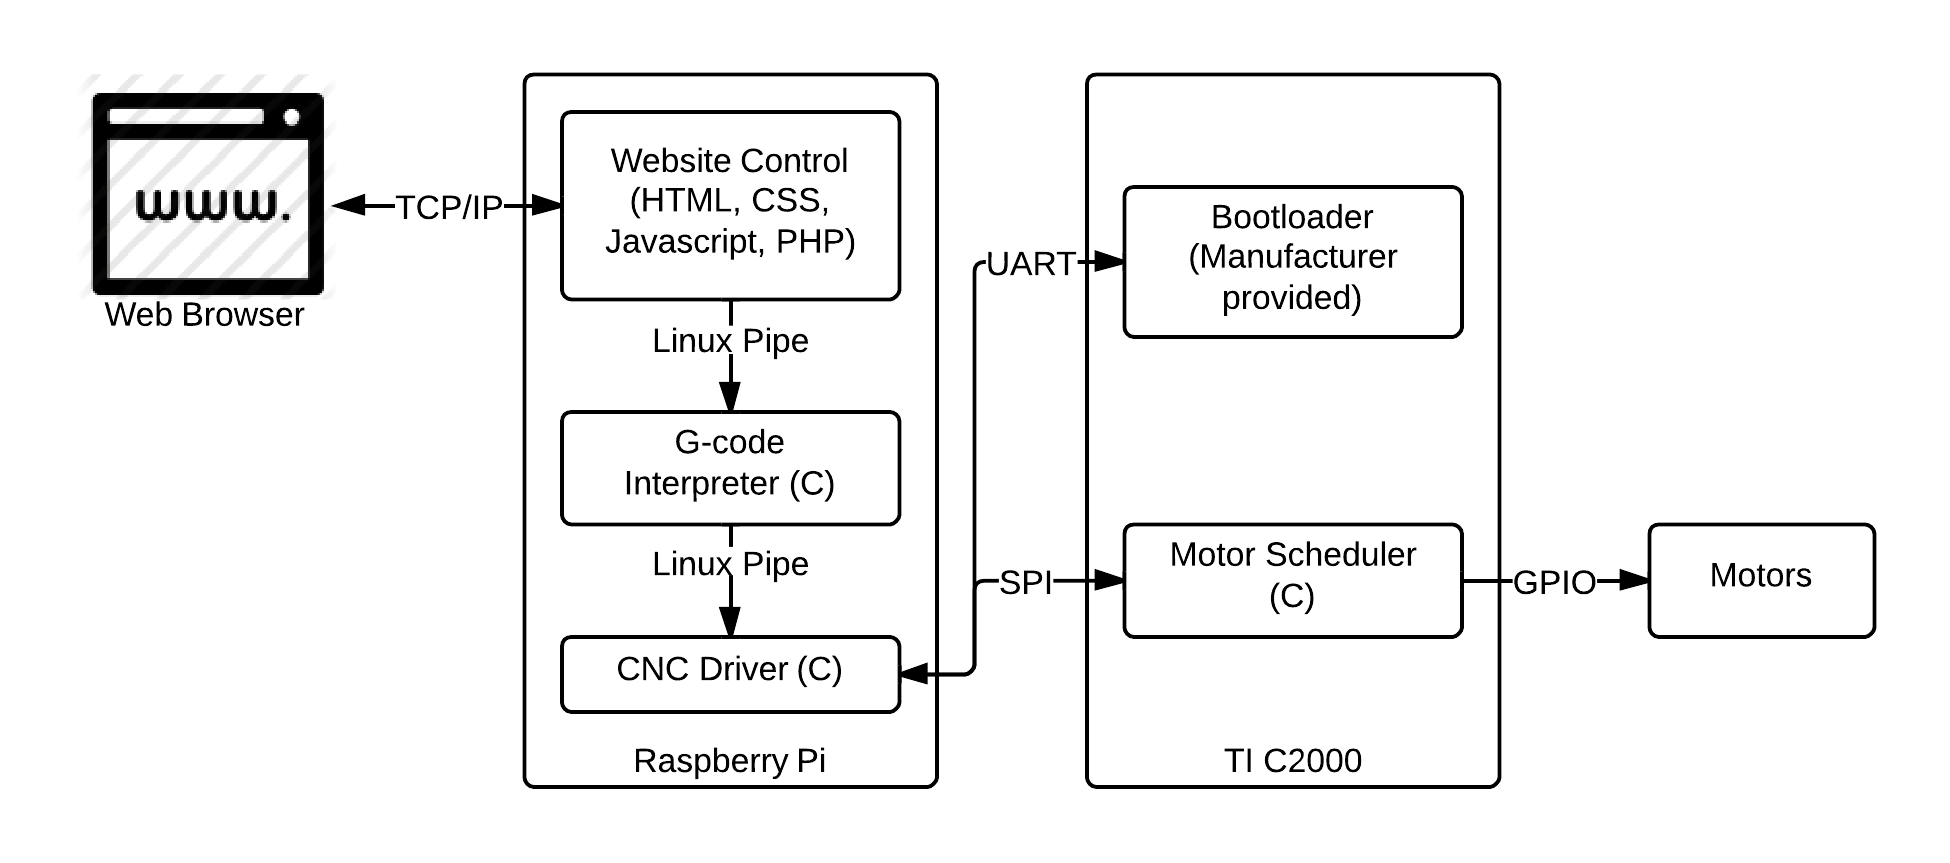
\includegraphics[width=1\textwidth]{software-design/firmware-hierarchy.png}
	\caption{Firmware Hierarchy}
	\label{fig:firmware-hierarchy}
\end{figure}
	\chapter{Schematic Functional Blocks}
\label{chap:schematic-breakdown}

\begin{figure}[h]
\centering
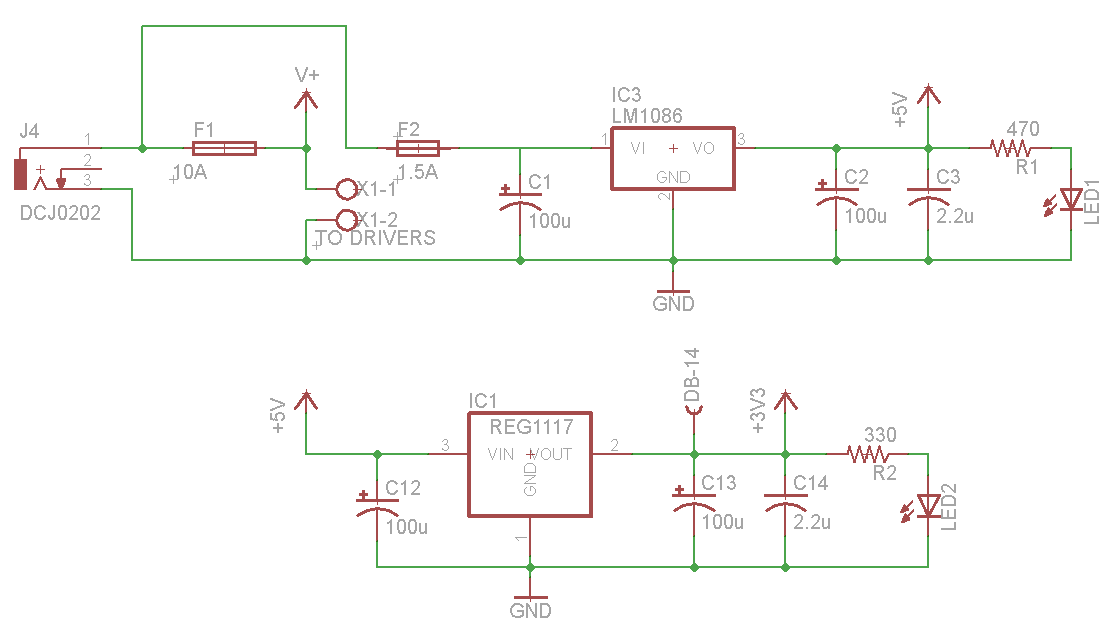
\includegraphics[width=0.6\textwidth]{reliability-analysis/functional-breakdown-power.png}
\caption{Power Regulation Block}
\label{fig:power-block}
\end{figure}


\begin{figure}[h]
\centering
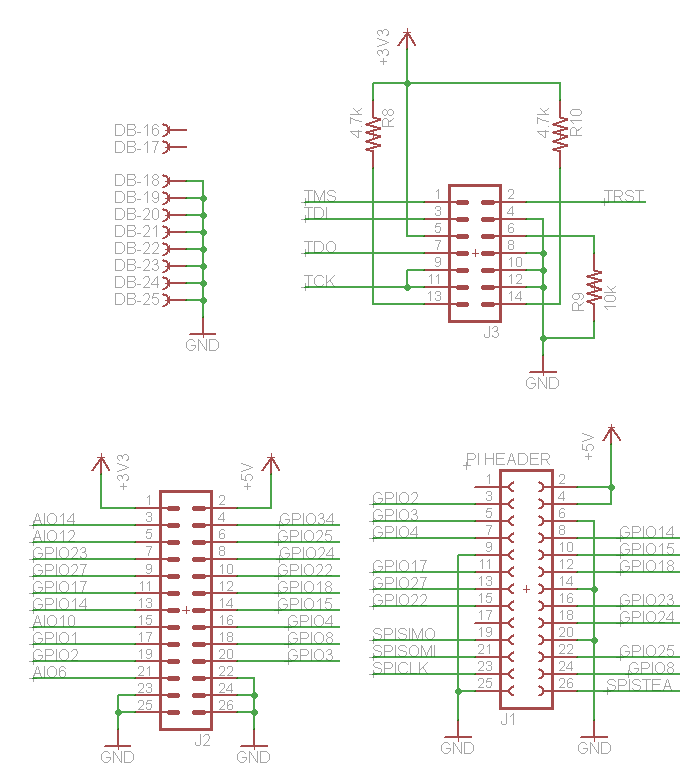
\includegraphics[width=0.5\textwidth]{reliability-analysis/functional-breakdown-connectors.png}
\caption{Off-Board Connectors Block}
\label{fig:connectors-block}
\end{figure}

\begin{figure}[h]
\centering
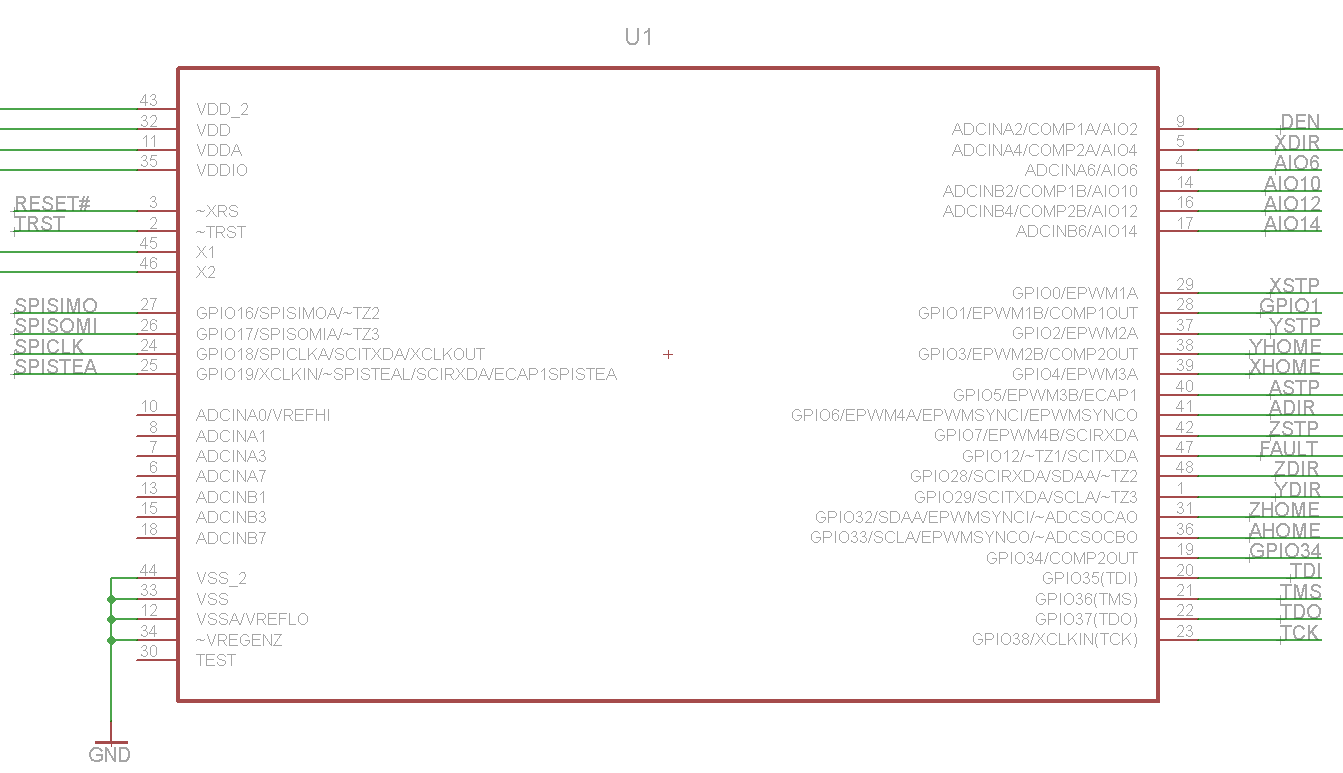
\includegraphics[width=\textwidth]{reliability-analysis/functional-breakdown-uc.png}
\caption{Microcontroller Block}
\label{fig:uc-block}
\end{figure}

\begin{figure}[h]
\centering
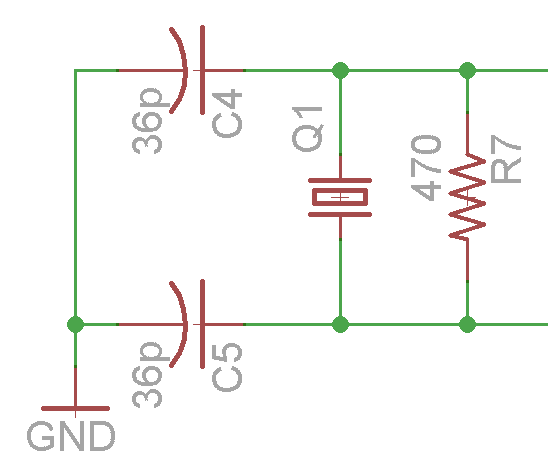
\includegraphics[width=0.5\textwidth]{reliability-analysis/functional-breakdown-crystal.png}
\caption{Crystal Block}
\label{fig:crystal-block}
\end{figure}


	\chapter{Failure Mode, Effects, and Criticality Analysis}

\begin{table}[h]
\caption{\gls{fmeca} Analysis}
\label{tab:fmeca}
\centering
{\scriptsize
\tabcolsep=0.1cm
\begin{tabular}{|m{2cm}|m{2cm}|m{2cm}|m{3cm}|m{1.7cm}|m{5cm}|}
\hline
	Functional Block & Failure Mode & Failure Cause & Effects & Criticality & Suggested Action \\ \hline
	Power Regulation & 5V rail voltage $>$5V & 5V regulator internal short & Destruction of 3.3V regulator and all microelectronics, including \gls{pi} & Critical & Choose a reliable 5V regulator, include over-voltage protection circuit. \\ \hline
	Power Regulation & 5V rail voltage $<$5V & 5V regulator internal open circuit & No microcontroller on system starts & Marginal & include instructions on replacing the 5V regulator \\ \hline
	Power Regulation & 3.3V rail voltage $>$3.3V & 3.3V regulator internal short & Destruction of all microelectronics on control board & Marginal & Choose a reliable 3.3V regulator, include over-voltage protection circuit \\ \hline
	Power Regulation & 3.3V rail voltage $<$3.3V & 3.3V regulator internal open circuit & Control board microcontroller does not start, \gls{pi} cannot connect to microcontroller & Marginal & Choose a reliable 3.3V regulator, include instructions on replacing the 3.3V regulator \\ \hline
	Off-Board Connectors & Open connection & Worn out connectors & Subsystems cannot communicate & Marginal & Design system so that disconnecting and reconnecting of connectors is not frequently required, include instructions on replacing the connectors \\ \hline
	Off-Board Connectors & Poor electrical connection & Worn out connectors & Poor inter-system communication & Marginal & Design system so that disconnecting and reconnecting of connectors is not frequently required, include instructions on replacing the connectors \\ \hline
	Off-Board Connectors & Short & Incorrect connection made & Damaged components, particularly power regulators & Marginal & Design system so that correct connection is as clear as possible and include detailed assembly instructions \\ \hline
	$\mu$Controller & Incorrect control pulses & Software error & \gls{cnc} accuracy less than expected & Negligible & Make firmware upgrades possible in-system through bootloader \\ \hline
	$\mu$Controller & Emergency button not registered & Hardware failure & \gls{cnc} not stopped when requested & Catastrophic & Create a system test to ensure that emergency button functions \\ \hline
	$\mu$Controller & Emergency button not registered & Software error & \gls{cnc} not stopped when requested & Catastrophic & Include watchdog timer with as short a period as possible that performs the same action as the emergency stop button \\ \hline
	Crystal & No oscillation & Electrical or mechanical shock to crystal & Control board microcontroller does not start & Marginal & Include handling and electrical shock prevention instructions, allow use of internal oscillator when external crystal fails \\ \hline
	Crystal & Increased Frequency & \gls{emi}\cite{emicrystal} & \gls{cnc} accuracy less than expected & Marginal & Create a system test to compare timing on the \gls{ti} microcontroller compared to the UTC fetched from the Internet on the \gls{pi}. \\ \hline
\end{tabular}
}
\end{table}
	\begin{thebibliography}{9}
%patent

\bibitem{cncpatent}
T. A-Tung, 
”CNC milling machine,” 
U.S. Patent 6,050,760 April 18, 2000

\bibitem{controlmethodpatent}
H. Kawamura, M. Miyata and R. Nozawa, 
”Numerical control method” 
U.S. Patent 4,591,968 May 27, 1986

\bibitem{navpatent}
A. Adamsbaum and J. Deschamps, 
”Navigational process and device for path control,” 
U.S. Patent 3,805,2610 April 16, 1974

\bibitem{executionpatent}
 T. Ichikawa, 
”Numerical control unit with set amount of execution,” 
U.S. Patent 8,036,770 October 11, 2011

\bibitem{webservicepatent}
S.K. Selvaraj and Z. Xiao, 
”Approach For Printing To Web Services-Enabled Printing Devices,” 
U.S. Patent 12/399,884 September 9, 2010

\bibitem{motorcontrolpatent}
S. Ushiyama and K. Matsumoto,  
”Control device of electric motor,” 
U.S. Patent 8,598,818 December 3, 2013

%software-design
\bibitem{piccolo}
	\textit{TMS320F2802x, TMS320F2802xx (Piccolo) MCUs},
	\gls{ti}, Dallas, TX,
	2013, pp. 16.
\bibitem{archlinux}
	\textit{Raspberry Pi | Arch Linux ARM},
	Arch Linux ARM,
	2014, pp. 1.

%economic
\bibitem{3dprintimpact}
	Richard A. D'Aveni,
	\textit{3-D Printing Will Change the World},
	Harvard Business Review, Boston, MA,
	March 2013, pp. 53-54,

\bibitem{3dprintsave}
	Heather Kelly,
	\textit{Study: At-home 3D printing could save consumers thousands},
	CNN Technology Review,
	July 31, 2013

%reliability-analysis
\bibitem{mil217f}
	\textit{Reliability Prediction of Electronic Equipment} (MIL-HDBK-217F), 5th ed.,
	Dept. of Defense, Washington, DC,
	1991, pp. 5-1 - 5-24.
\bibitem{picollo}
	\textit{TMS320F2802x, TMS320F2802xx (Piccolo) MCUs},
	\gls{ti}, Dallas, TX,
	2013, pp. 81, 123.
\bibitem{oki78sr}
	\textit{OKI-78SR Series Fixed Output 1.5 Amp SIP DC/DC Converters},
	Murata Power Solutions, Mansfield, MA,
	2013, pp. 1-3.
\bibitem{lm1117}
	\textit{LM1117-N/LM1171 800mA Low-Dropout Linear Regulator},
	\gls{ti}, Dallas, TX,
	2013, pp. 2, 5.
\bibitem{ieeec951}
	\textit{\gls{ieee} Standard for Safety Levels with Respect to Human Exposure to Radio Frequency Electromagnetic Fields, 3kHz to 300GHz} (\gls{ieee} Std C95.1), 2nd ed.,
	\gls{ieee}, New York, NY,
	2005, pp. 20-25.
\bibitem{ieeenesc}
	\textit{National Electrical Safety Code},
	\gls{ieee}, New York, NY,
	2007, pp 17-20, 32-57.
\bibitem{mil882d}
	\textit{Standard Practice for System Safety} (MIL-STD-882D), 4th ed.,
	Dept. of Defense, Washington, DC,
	2000, pp. 18-20.
\bibitem{emicrystal}
	\textit{EMI-Induced Failures in Crystal Oscillators},
	\gls{ieee} Transactions, vol. 33, no. 4, New York, NY,
	1991, pp. 334-341.

%environmental
\bibitem{3dprintsustain}
	Dr. Philip Reeves,
	\textit{Additive Manufacturing – A supply chain wide response to economic uncertainty and environmental sustainability},
	Econolyst Limited, The Silversmiths, Crown Yard, Wirksworth, Derbyshire, UK
	2013
\bibitem{3dprintenvironment}
	Pearce M. Krieger,
	\textit{"Environmental Life Cycle Analysis of Distributed Three-Dimensional Printing and Conventional Manufacturing of Polymer Products"},
	ACS Sustainable Chemistry \& Engineering: 131002082320002. doi:10.1021,
	2013	

%development analysis
\bibitem{dev_intelligent}
	\textit{Intelligent Stepper Motor Driver with DRV8811/18/24/25},
	\gls{ti}, Dallas, TX,
	2013, pp. 22.
\bibitem{dev_peripherals}
	\textit{Programming TMS320x28xx and 28xxx Peripherals in C/C++},
	\gls{ti}, Dallas, TX,
	2013, pp. 189.
\bibitem{dev_optimize}
	\textit{TMS320C28x Optimizing C/C++ Compiler v6.2.4},
	\gls{ti}, Dallas, TX,
	2013, pp. 24.
\bibitem{dev_drv}
	\textit{DRV8811/18/24/25 Datasheet},
	\gls{ti}, Dallas, TX,
	2013, pp. 22.
\end{thebibliography}

\end{appendices}
\end{document}
